%**************************************************
% Document Class Definition
% **************************************************
\documentclass[%
	paper=A4,				% paper size --> A4 is default in Germany
	twoside=true,				% onesite or twoside printing
	openright,				% doublepage cleaning ends up right side
	parskip=full,				% spacing value / method for paragraphs
	chapterprefix=true,			% prefix for chapter marks
	11pt,					% font size
	headings=normal,			% size of headings
	bibliography=totoc,			% include bib in toc
	listof=totoc,				% include listof entries in toc
	titlepage=on,				% own page for each title page
	captions=tableabove,			% display table captions above the float env
	draft=false,				% value for draft version
]{scrreprt}%
%\documentclass{article}

\usepackage[utf8]{inputenc}
\usepackage[english]{babel}

\newcommand{\thesisTitle}{Topics in Computer Vision subtitle}
\newcommand{\thesisName}{Vadim Kantorov}
\newcommand{\thesisSubject}{Documentation}
\newcommand{\thesisDate}{April 7, 2014}
\newcommand{\thesisVersion}{0.2.3}

\newcommand{\thesisFirstReviewer}{Jane Doe}
\newcommand{\thesisFirstReviewerUniversity}{\protect{Clean Thesis Style University}}
\newcommand{\thesisFirstReviewerDepartment}{Department of Clean Thesis Style}

\newcommand{\thesisSecondReviewer}{John Doe}
\newcommand{\thesisSecondReviewerUniversity}{\protect{Clean Thesis Style University}}
\newcommand{\thesisSecondReviewerDepartment}{Department of Clean Thesis Style}

\newcommand{\thesisFirstSupervisor}{Ivan Laptev}
\newcommand{\thesisSecondSupervisor}{Minsu Cho}

\newcommand{\thesisUniversity}{\protect{École Normale Supérieure}}
\newcommand{\thesisUniversityDepartment}{Department of Clean Thesis Style}
\newcommand{\thesisUniversityInstitute}{Institut for Clean Thesis Dev}
\newcommand{\thesisUniversityGroup}{Clean Thesis Group (CTG)}
\newcommand{\thesisUniversityCity}{City}
\newcommand{\thesisUniversityStreetAddress}{Street address}
\newcommand{\thesisUniversityPostalCode}{Postal Code}

\DeclareOldFontCommand{\rm}{\normalfont\rmseries}{\mathrm}
\DeclareOldFontCommand{\bf}{\normalfont\bfseries}{\mathbf}
\newcommand{\etal}{\textit{et al}.}
\newcommand{\ie}{\textit{i}.\textit{e}., }
\newcommand{\eg}{\textit{e}.\textit{g}.}
\newcommand\vadimkantorov[1]{\textcolor{blue}{[VK: #1]}}
\def\fixme#1{\textcolor{red}{[#1]}\marginpar{\textcolor{red}{FIXME}}}
\def\checked#1{#1}

%\usepackage{xcolor}
%\definecolor{darkgreen}{rgb}{0,0.5,0}


% https://ctan.math.illinois.edu/macros/latex/contrib/cleanthesis/doc/cleanthesis-doc.pdf
\usepackage[					% clean thesis style
	figuresep=colon,%
	sansserif=false,%
	hangfigurecaption=false,%
	hangsection=true,%
	hangsubsection=true,%
	colorize=full,%
	colortheme=bluemagenta,%
        bibsys=bibtex,%
        configurebiblatex=false,%
	bibfile=thesis,
]{cleanthesis}

%\usepackage[pagebackref=true,breaklinks=true,letterpaper=true,colorlinks,urlcolor=blue,bookmarks=false]{hyperref}

\hypersetup{				% setup the hyperref-package options
	pdftitle={\thesisTitle},	% 	- title (PDF meta)
	pdfsubject={\thesisSubject},	% 	- subject (PDF meta)
	pdfauthor={\thesisName},	% 	- author (PDF meta)
	plainpages=false,		% 	- 
	colorlinks=false,		% 	- colorize links?
	pdfborder={0 0 0},		% 	-
	breaklinks=true,		% 	- allow line break inside links
	bookmarksnumbered=true,		%
	bookmarksopen=true		%
}

\usepackage{pdfpages}
\usepackage{calc}
\usepackage{xcolor}
\usepackage{mdframed}
\usepackage{times}
\usepackage{epsfig}
\usepackage{graphicx}
\usepackage{amsmath}
\usepackage{amssymb}
\usepackage{multirow}
\usepackage{array}
\usepackage{graphicx}
\usepackage{booktabs}
\usepackage{color}
\usepackage{marvosym}
\usepackage{adjustbox}
\usepackage{cite}

\title{Topics in Computer Vision: efficient video features and weakly-supervised object detection}
\author{Vadim Kantorov}
\date{2023}

\begin{document}
\selectlanguage{english}

% --------------------------
% Front matter
% --------------------------
\pagenumbering{roman}			% roman page numbing (invisible for empty page style)
\pagestyle{empty}				% no header or footers


\begin{titlepage}

\includepdf{front.pdf}
%\cleardoublepage % pour laisser une page blanche au verso de la page de garde
\newpage
\vspace*{\fill}
\noindent\begin{center}
\begin{minipage}[t]{(\textwidth-2cm)/3+1cm}
École normale supérieure \\
45 rue d'Ulm \\
75005 Paris
\end{minipage}
%
\hfill
%
\begin{minipage}[t]{(\textwidth-2cm)/3-1cm}
Inria Paris \\
2 rue Simone Iff \\
75012 Paris
\end{minipage}
%
\hfill
%
\begin{minipage}[t]{5.5cm}
UPMC\\
Ecole Doctorale de Sciences\\
Math\'ematiques de Paris Centre\\
4 place Jussieu\\
75252 Paris Cedex 05\\
Boite courrier 290
\end{minipage}
\end{center}
\end{titlepage}
%\maketitle
\cleardoublepage



\pagestyle{plain}				% display just page numbers
\pdfbookmark[0]{Abstract}{Abstract}
\chapter*{Abstract}
\label{sec:abstract}
\vspace*{-10mm}
Abstract in English

\newpage
{\usekomafont{chapter}Résumé}\label{sec:abstract-fr} \\
Abstract en français

\cleardoublepage



\pdfbookmark[0]{Acknowledgement}{Acknowledgement}
\chapter*{Acknowledgement}
\label{sec:acknowledgement}
\vspace*{-10mm}
My acknowledgements

\cleardoublepage

\setcounter{tocdepth}{1}
\tableofcontents
\cleardoublepage

% --------------------------
% Body matter
% --------------------------
\pagenumbering{arabic}			% arabic page numbering
\setcounter{page}{1}			% set page counter
\pagestyle{maincontentstyle} 		% fancy header and footer


\chapter{Introduction}
This thesis describes three research projects I worked on during 2012-2022:
\begin{enumerate}
\item Video clip classification using motion vectors estimated by video codecs at encoding time for speeding-up motion feature computation
\item Weakly-supervised object detection using contast cue as guidance
\item Pretraining the detection head in addition to the backbone for improving object detection and instance segmentation
\end{enumerate}



\chapter{Related work}
My related work



\chapter{Efficient feature extraction, aggregation and classification for action recognition}
\section{Introduction}
\begin{abstract}Local video features provide state-of-the-art performance for action recognition. While the accuracy of action recognition has been continuously improved over the recent years, the low speed of feature extraction and subsequent recognition prevents current methods from scaling up to real-size problems. We address this issue and first develop highly efficient video features using motion information in video compression. We next explore feature encoding by Fisher vectors and demonstrate accurate action recognition using fast linear classifiers. Our method improves the speed of video feature extraction, feature encoding and action classification by two orders of magnitude at the cost of minor reduction in recognition accuracy. We validate our approach and compare it to the state of the art on four recent action recognition datasets.
\end{abstract}
The amount of video has increased dramatically over recent years and continues to grow. Striking indications of this development
include 6000 years of video uploaded to YouTube
yearly\footnote{\scriptsize
\url{http://youtube.com/t/press\_statistics}} and millions of
surveillance cameras installed only in the UK. According to
Cisco\footnote{\scriptsize
\url{http://newsroom.cisco.com/dlls/2010/prod_060210.html}},
video is expected to dominate Internet traffic by 91\% in 2014.
%, or a webcam network installed for public monitoring of Russian elections that has generated over 100 years of video just in one day\footnote{http://www.rostelecom.ru/en/ir/news/d212878}.

The access to information in such gigantic quantities of video
data requires accurate and efficient methods for automatic video analysis. Much work has been recently devoted to automatic video understanding and recognition of human actions in
particular~\cite{Laptev08,Liu11,Niebles10,Sadanand12,Schuldt04,Wang12}.
While the recognition accuracy has been continuously improved,
current methods remain limited to relatively small datasets due
to the low speed of video processing, often ranging in the order of 1-2 frames per second. This stands in a sharp contrast with
the needs of large-scale video indexing and retrieval in modern
video archives. Fast video recognition is also required by
client applications, e.g., for automatic on-the-fly video
moderation and video editing. Efficient video representations
enabling fast event recognition will also foster solutions to
new problems such as automatic clustering of very large video
collections.

The main goal of this work is efficient action recognition. We
follow the common bag-of-features action recognition
pipeline~\cite{Laptev08,Schuldt04,Wang12} and explore the speed
and memory trade-offs of its main steps, namely, feature
extraction, feature encoding and classification. Given their
success for action recognition, we represent video
using motion-based HOF~\cite{Laptev08} and MBH~\cite{Wang12}
local descriptors. Motion estimation at dense grid, however, is
a time-consuming process that
limits the speed of feature extraction.
In this work we avoid motion estimation and design
fast
descriptors using motion information from video compression.
In contrast to the dense optical flow (OF), video compression
provides sparse motion vectors only (we call it MPEG~flow).
As one contribution of this paper, we show that the use of
sparse MPEG flow instead of the dense OF improves the speed of
feature extraction by {\em two orders of magnitude} and implies
only minor reduction in classification performance.

Feature encoding typically involves assignment of local
descriptors to one or several nearest elements in a visual
vocabulary. Given the large number of video descriptors, the
speed of this step is a major bottleneck. We evaluate using
kd-forest approximate nearest neighbor search \cite{Philbin07}
and analyze the associated trade-off between the speed and
recognition accuracy. We next investigate Fisher vector (FV)
encoding~\cite{Perronnin12} and show improved action recognition while using fast linear classifiers.
We evaluate the speed and accuracy of our approach on
\mbox{Hollywood-2}~\cite{Marszalek09}, UCF50~\cite{Reddy12},
HMDB51~\cite{Kuehne11} and UT-Interaction~\cite{Ryoo10}
benchmarks. The implementation of out method is available at~\cite{projectpage}.

The rest of the paper is organized as follows. 
After reviewing related work in Section~\ref{sec:relatedwork} we address efficient extraction of local video features in
Section~\ref{sec:features}. Section~\ref{sec:quantization}
describes our fast video encoding.
Section~\ref{sec:experiments} presents experimental results.

\section{Related work}\label{sec:relatedwork}
Recent methods show significant progress towards action
recognition in realistic and challenging videos from YouTube,
movies and
TV~\cite{Laptev08,Laptev07,Liu11,Niebles10,Rodriguez08,Sadanand12,Wang12}.
Among other approaches, bag-of-features (BOF)
methods~\cite{Dollar05,Laptev05,Schuldt04} have gained
popularity due to their simplicity, wide range of application
and high recognition accuracy.
BOF methods represent actions by collections of local space-time descriptors aggregated over the video.
Several alternative local descriptors have been proposed
including histograms of flow orientations (HOF)~\cite{Laptev08},
histograms of 3D gradients
(HOG3D)~\cite{klaser2008spatio,Scovanner07}, motion boundary
histograms (MBH)~\cite{Dalal06,Wang12}, shapes of point
trajectories~\cite{Matikainen09,Messing09,Wang12}, local trinary patterns~\cite{Kliper12,Yeffet09} and others. 
Mid-level features such as action attributes~\cite{Liu11} and action
bank~\cite{Sadanand12} have also been explored. Recent
 evaluation~\cite{Wang12} demonstrates that MBH, HOF
and HOG descriptors sampled along dense point trajectories
outperform other
methods on a number of challenging datasets~\cite{Wang12}. 
More recent extensions demonstrate improvements using motion stabilization and person trajectories~\cite{Jain13,Wang13}.
We follow~\cite{Wang12} and design a new motion-based local
descriptor that drastically improves the speed of previous
methods at the cost of minor decrease in the recognition
accuracy.

%sampling of feature   required for larger scale problems. Random sampling
%of dense features locations~\cite{Feng13} has been studied as
%well, it leads to feature extraction substantially faster than
%\cite{Wang12}, but several times slower than this work. 


Efficient action recognition has been addressed by several
methods. The work~\cite{mpeg3,mpeg2,mpeg1} is particularly
related to ours as it makes use of motion information from video compression for fast action recognition. This previous work,
however, designs action-specific descriptors and, hence, its
speed scales linearly with the number of action classes. In
contrast, we design a generic action representation and evaluate its accuracy and efficiency on many action classes in
challenging settings.
Yeffet and Wolf~\cite{Yeffet09} extend the fast LBP image
descriptor to a Local Trinary Pattern (LTP) descriptor in video
and evaluate its accuracy on action recognition. While LTP was
claimed to run in real time, no quantitative evaluation of its
speed was reported in~\cite{Yeffet09}. Differently to LTP, we
use flow-based MBH and HOF descriptors which have recently shown excellent results for action recognition~\cite{Wang12}. Yu
et~al.~\cite{Yu10} have proposed another pixel-based local
descriptor for efficient action recognition. We quantitatively
compare our method with~\cite{Yu10} and show improvements in
both the speed and accuracy.
Closely related to our work, \cite{Feng13} has 
recently improved the speed of local feature extraction in video
by random feature sampling.
We experimentally compare our method to~\cite{Feng13}
and show one order of magnitude improvement in speed while 
also demontrating improved accuracy.


Alternative schemes for feature encoding
%, i.e.~aggregation of local descriptors into global representations,
have been recently evaluated for image classification
in~\cite{Chatfield11}.
%While histogram encoding is the most common one, 
Fisher vector (FV) encoding~\cite{Perronnin10} has been shown to provide best accuracy using efficient linear kernels for
classification. FV encoding has been successfully applied for
event detection \cite{Revaud13} and we are confirming its
improved performance and efficiency compared to the
histogram encoding typically used in action recognition. We also investigate efficient computation of FV using approximate
nearest neighbor methods for descriptor assignment. FV encoding enables high recognition accuracy using fast linear
classifiers which is a big advantage for large-scale video
recognition. \smallskip

\noindent\textbf{Contributions.} The contributions of this work are the following. First, we design and thoroughly evaluate an efficient motion descriptor based on the video compression which is 100x faster to compute at a minor degradation of recognition performance compared to the state-of-the-art~\cite{Wang12}. Second, to the best of our knowledge, we are the first to evaluate both efficiency and classification performance of FV and VLAD for action recognition and find it improving the recognition rates without loss in speed compared to the histogram encoding.



%%%%%%%%%%%%%%%%%%%%%%%%%%%%%%%%%%%%%%%%%%%%%%%%%%%%%%%%%%%%%%%%
%%%%%%%%%%%%% Video encoding
%%%%%%%%%%%%%%%%%%%%%%%%%%%%%%%%%%%%%%%%%%%%%%%%%%%%%%%%%%%%%%%%
\section{Descriptor encoding}
\label{sec:quantization}
The purpose of descriptor encoding is to transform collections of local image or video descriptors $\left\{\textbf{x}_i\dots\textbf{x}_N\right\}$ into fixed-size vector representations.
In this paper we investigate three different descriptor encoding schemes and propose their computational improvements as described below.

\subsection{Histogram encoding}
\label{subsec:histenc}
Histogram encoding is a common method for representing video by local descriptors. First, for each descriptor type (HOG, HOF, MBHx, MBHy) a vocabulary of $K$ visual words is constructed using K-means. Then each descriptor is assigned to one of the visual words and the visual word indices are accumulated in a histogram. We follow~\cite{Laptev08} and use ``space-time pyramid'' which allows to capture the rough spatial and temporal layout of action elements. We split videos into six spatio-temporal grids ($x\times y \times t$: 1x1x1, 2x2x1, 1x3x1, 1x1x2, 2x2x2, 1x3x2, a total of 24 cells). In total we have $C=96\text{ channels} = 4 \text{ descriptor types}\times 24\text{ cells}$, that is one channel per a pair of descriptor type and grid cell. Each cell accumulates its own histogram which is then $l_1$-normalized, thus the total histogram representation is of size $C\cdot K$. We also employ space-time pyramids for the Fisher vector and VLAD encoding methods described in Sections \ref{subsec:fvenc} and \ref{subsec:vladenc} respectively.

For visual word assignment we experimented with using brute-force nearest neighbors and with using the kd-trees from the FLANN library \cite{Muja09}. The motivation for using kd-trees is the significant improvement in processing speed over the brute-force algorithm (see Subsection~\ref{subsec:descencimprov}). The main parameters for the kd-trees method are the number of trees and the number of tests  made during the descent over trees. 

\subsection{Fisher Vector}
\label{subsec:fvenc}
Fisher Vector (FV) has been reported to consistently improve the performance in image classification and image retrieval tasks~\cite{Jegou12}.
Another advantage of FV encoding over histogram encoding is it's good performance using fast linear classifiers.
FV encoding assumes that descriptors are generated by a GMM model with diagonal covariance matrices. Similarly to histogram encoding, the GMM model of $K$ Gaussians is first learned on the training set. 
Once the model $\left(\boldsymbol\mu_k, \boldsymbol\sigma_k\right)$ is learned, the FV representation of the descriptors $\left\{\textbf{x}_1\dots \textbf{x}_N\right\}$ is given by the two parts \cite{Perronnin10}:
$${\textbf u}_k = \frac{1}{N\sqrt{\pi_k}}\sum_{i=1}^{N}q_{ki}\left(\frac{\textbf{x}_i-\boldsymbol\mu_k}{\boldsymbol\sigma_k}\right)$$

\begin{equation}
\label{eq:fv_vk}
\textbf{v}_k=\frac{1}{N\sqrt{2\pi_k}}\sum_{i=1}^{N}q_{ki}\left[\left(\frac{\textbf{x}_i-\boldsymbol\mu_k}{\boldsymbol\sigma_k}\right)^2-\textbf{1}\right]
\end{equation}
where $q_{ki}$ is the Gaussian soft assignment of the descriptor $\textbf{x}_i$ to the $k$-th Gaussian, $\pi_k$ are the mixture weights, division and square are term-by-term operations. The \textbf{u} part captures the first-order differences, the \textbf{v} part captures the second-order differences. The final representation of size $C\cdot 2DK$ is given by concatenation of the two parts. As suggested in \cite{Perronnin10}, we then take signed square root and $l_2$-normalize the result. We apply the same normalization scheme to VLAD, described next.
\subsection{VLAD}
\label{subsec:vladenc}
The VLAD encoding is the simplified version of Fisher vector which considers only the first-order differences and assigns descriptors to a single mixture component. It was also shown to outperform the histogram encoding in~\cite{Jegou12}. In our implementation we keep the soft-assignment factor $q_{ki}$. The VLAD representation of size $C\cdot DK$ is then given by concatenating:$$\textbf{u}_k=\sum_{i : NN\left(\textbf{x}_i\right)=\boldsymbol\mu_k}q_{ki}\left(\textbf{x}_i -\boldsymbol\mu_k\right)$$



%%%%%%%%%%%%%%%%%%%%%%%%%%%%%%%%%%%%%%%%%%%%%%%%%%%%%%%%%%%%%%%%
%%%%%%%%%%%%% Efficient video features
%%%%%%%%%%%%%%%%%%%%%%%%%%%%%%%%%%%%%%%%%%%%%%%%%%%%%%%%%%%%%%%%
\section{Efficient video features}
\label{sec:features}

Dense Trajectory (DT) features together with MBH and HOF descriptors achieve state-of-the-art accuracy in action recognition~\cite{Wang12} at the cost of high computational requirements.
%but are limited in speed with the current implementation being able to process one or a few frames per second depending on video resolution. 
%Currently available implementation of Dense Trajectory (DT) features provided by the authors of~\cite{Wang12} can process approximately one video frame per second. 
The analysis in~\cite{Wang12} indicates that most of the running time ($61\%$) is spent on the computation of optical flow, while the second most expensive operation ($36\%$) is aggregation of dense flow measurements into histogram descriptors (discarding the "save features to disk" part). In this paper we alleviate the expense of both of these steps by (i) re-using motion estimates available from video compression and (ii) constructing descriptors from very sparse motion measurements. %, typically available only on a $16\times16$ pixel grid in standard video compression schemes.
In this section we first analyze the quality of motion vectors available in compressed video representations and then describe our efficient video descriptor.

%This section describes and motivates the design of our video descriptor. We first review existing descriptors and outline their strengths and limitations. We then analyze the properties of the motion field available in compressed video representations and use it to construct a new video descriptor.

%\subsection{Local video descriptors}

%Local video descriptors~\cite{Dollar05,Laptev05,Schuldt04} have been shown successful for recognizing events in realistic videos such as movies and TV footage. Several descriptors have been proposed capturing local histograms of 2D gradients (HOG) and flow orientations(HOF)~\cite{Laptev08}, histograms of 3D gradients (HOG3D)~\cite{Scovanner07,klaser2008spatio}, motion boundary histograms (MBH)~\cite{Dalal06,Wang12}, local shapes of point trajectories~\cite{Matikainen09,Messing09,Wang12} and local trinity patterns~\cite{Yeffet09,Kliper12}. Intermediate-level features such as attributes~\cite{Liu11} and pre-trained action bank detectors~\cite{Sadanand12} have also been explored. Recent comprehensive evaluation~\cite{Wang12} suggests that MBH, HOF and HOG descriptors densely sampled along point trajectories result in excellent performance and outperforms other methods on a large number of existing action recognition benchmarks. In particular, as we re-confirm in Section~\ref{sec:experiments}, MBH and HOF motion descriptors provide crucial contributions to the recognition performance.




\begin{figure*}[t!]
\begin{center}
\hspace*{-.3cm}
\begin{tabular}{p{.45\textwidth}p{.5\textwidth}p{.05\textwidth}}
\mbox{}\vspace{-2.5cm}\newline
\hspace*{1cm}{\small Sample frame from MPI Sintel dataset~\cite{Butler12}}\vspace{.07cm}\newline
%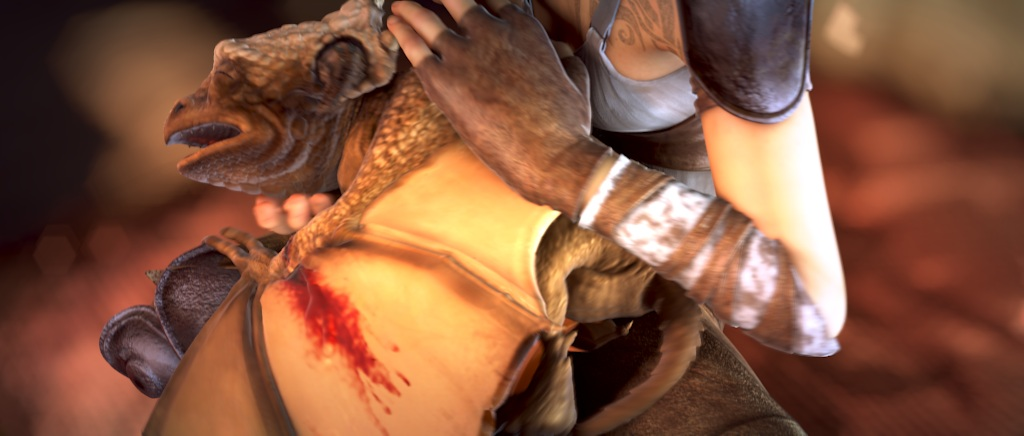
\includegraphics[trim=2cm 0cm 3cm 0cm, clip=true, width=.85\linewidth]{cvpr14_figures/flow/bandage_1_frame_0010.jpg}$\,\,$
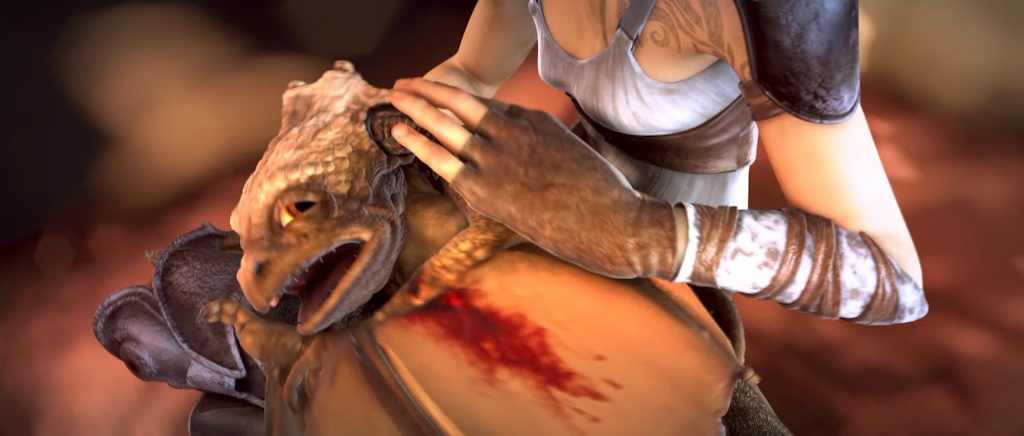
\includegraphics[trim=2cm 0cm 3cm 0cm, clip=true, width=.95\linewidth]{cvpr14_figures/flow/bandage_1_frame_0020.jpeg}$\,\,$
&
\hspace*{-.9cm}
\begin{tabular}{cc}
\small Quantized ground truth flow & \small Quantized MPEG flow, err=$0.283$\\
%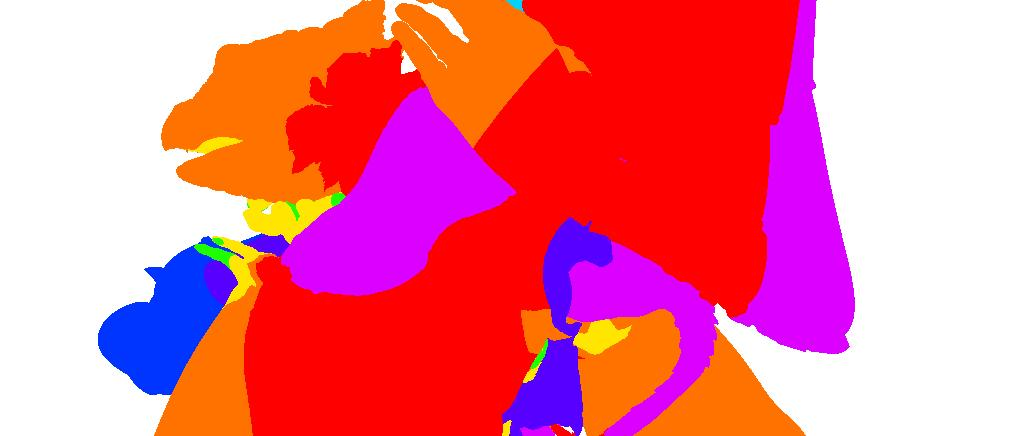
\includegraphics[width=.4\linewidth]{cvpr14_figures/flow/flow_bandage_1_frame011_orig_quant.jpeg} \vspace{.05cm}&
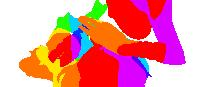
\includegraphics[width=.45\linewidth]{cvpr14_figures/flow/flow_bandage_1_frame021_orig_quant.jpeg} \vspace{.05cm}&
%
\includegraphics[width=.4\linewidth]{cvpr14_figures/flow/flow_bandage_1_frame011_mpeg_quant.png}  \vspace{.05cm}\\

\includegraphics[width=.45\linewidth]{cvpr14_figures/flow/flow_bandage_1_frame021_mpeg_quant.png}  \vspace{.05cm}\\
\small Quant. LK flow, err=$0.334$ & \small Quant. Farneb\"ack flow, err=$0.286$ \\
%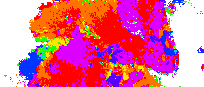
\includegraphics[width=.4\linewidth]{cvpr14_figures/flow/flow_bandage_1_frame011_stip_quant.png}  \vspace{.05cm}&
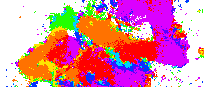
\includegraphics[width=.45\linewidth]{cvpr14_figures/flow/flow_bandage_1_frame021_stip_quant.png}  \vspace{.05cm}&
%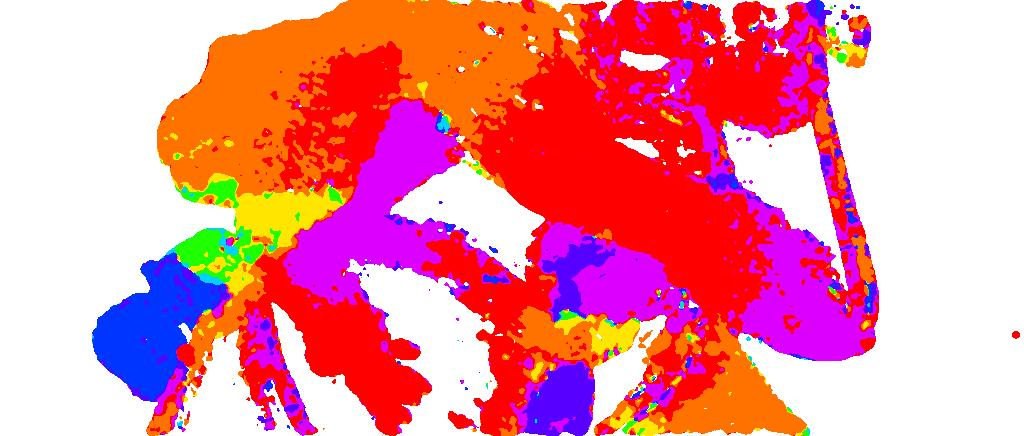
\includegraphics[width=.4\linewidth]{cvpr14_figures/flow/flow_bandage_1_frame011_traj_quant.jpeg} \vspace{.1cm}\\
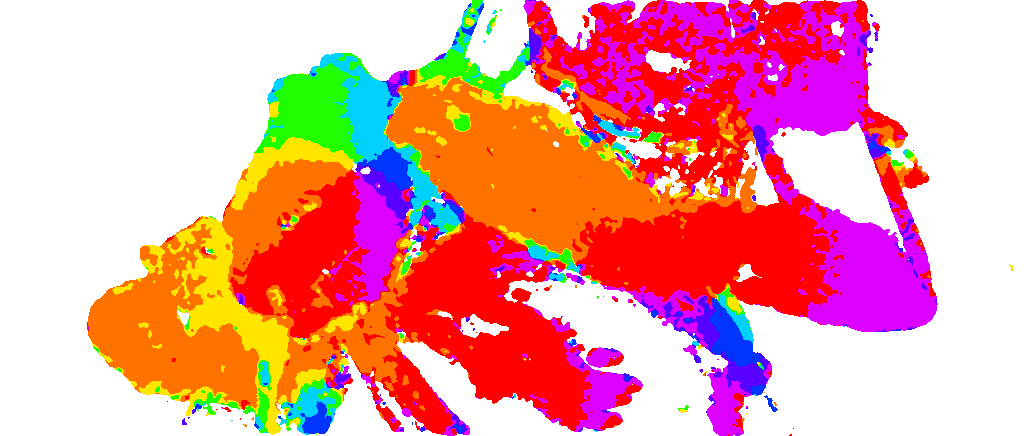
\includegraphics[width=.45\linewidth]{cvpr14_figures/flow/flow_bandage_1_frame021_traj_quant.png} \vspace{.1cm}\\
\end{tabular}
&
\mbox{}\vspace{1cm}\newline
\hspace*{-1.1cm}
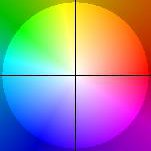
\includegraphics[width=1\linewidth]{cvpr14_figures/flow/flowcolorcode_reoriented.jpg}\vspace{.05cm}
\end{tabular}
\caption[Comparison of optical flow estimation]{Comparison of optical flow estimation for a synthetic video sequence ``bandage\_1'' from MPI Sintel dataset~\cite{Butler12}. On the right we compare the ground truth flow with the flow obtained from DivX video compression (MPEG flow) as well as optical flow estimated with Lukas-Kanade~\cite{Lucas81} and Farneb\"ack~\cite{Farneback03} methods. The direction of flow vectors is quantized into eight equally distributed orientations and is color-coded according to the color-wheel on the bottom-right. White color represents no motion. The error of the flow is obtained by the ratio of incorrectly quantized flow values when compared to the ground truth and evaluated over the whole video. While the resolution of MPEG flow is lower compared to other methods, the accuracy of all three methods is comparable both quantitatively and qualitatively.
%Left, top-to-bottom: ground truth flow; motion vectors from MPEG4 video compression; Lukas-Kanade flow (EPE)~\cite{Lucas81} and Farneb\"ack flow~\cite{Farneback03}. The accuracy of MPEG4, LK and Farneb\"ack motion fields are evaluated using endpoint error~\cite{Otte94}. Right: motion estimates quantized into eight orientation bins and one ``no-motion'' bin. Error indicates the mean disagreement of quantization between ground truth flow and the three flow estimates. Note that the EPE and the quantization error of MPEG4 flow are comparable to the errors of optical flow algorithms. The flow is color-coded according to the color-wheel on the top-right.
}
%\mbox{}\vspace{-.6cm}\\
\label{fig:flow1}
\end{center}
\end{figure*}


\begin{figure*}[t!]
\begin{center}
\hspace*{-.2cm}
\begin{tabular}{cccc}
\small Original movie frame & \small Quantized MPEG flow & \small Quantized LK flow & \small Quantized Farneb\"ack flow \\

\includegraphics[width=.23\textwidth]{cvpr14_figures/flow/actioncliptrain00009_0010bright.jpg} &

\includegraphics[width=.23\textwidth]{cvpr14_figures/flow/flow_actioncliptrain00009_frame010_mpeg_quant.png} & 

\includegraphics[width=.23\textwidth]{cvpr14_figures/flow/flow_actioncliptrain00009_frame010_stip_quant.png} &
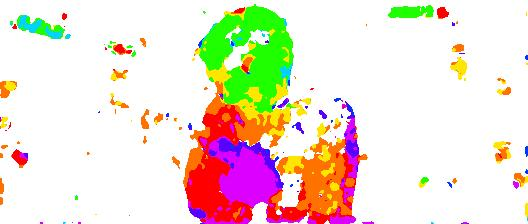
\includegraphics[width=.23\textwidth]{cvpr14_figures/flow/flow_actioncliptrain00009_frame010_traj_quant.jpeg}\\

\includegraphics[width=.23\textwidth]{cvpr14_figures/flow/flow_actioncliptest00686_frame010.jpeg} & 

\includegraphics[width=.23\textwidth]{cvpr14_figures/flow/flow_actioncliptest00686_frame010_mv_quant.png} & 
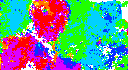
\includegraphics[width=.23\textwidth]{cvpr14_figures/flow/flow_actioncliptest00686_frame010_stip_quant.png} & 
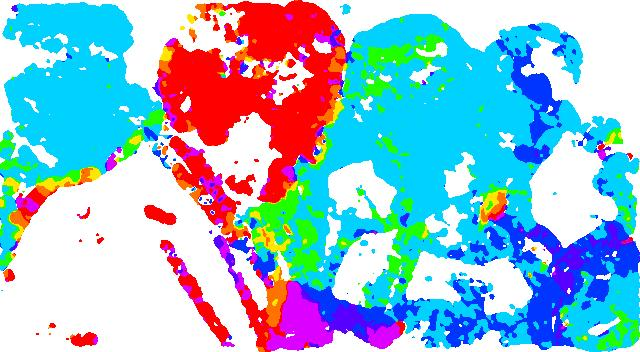
\includegraphics[width=.23\textwidth]{cvpr14_figures/flow/flow_actioncliptest00686_frame010_traj_quant.jpeg} \\
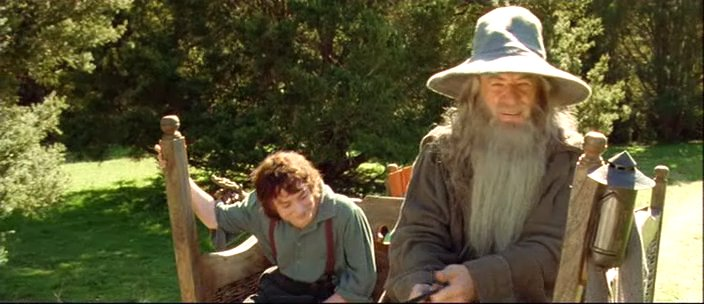
\includegraphics[width=.23\textwidth]{cvpr14_figures/flow/flow_actioncliptest00538_frame014.jpeg} & 

\includegraphics[width=.23\textwidth]{cvpr14_figures/flow/flow_actioncliptest00538_frame014_mv_quant.png} & 

\includegraphics[width=.23\textwidth]{cvpr14_figures/flow/flow_actioncliptest00538_frame014_stip_quant.png} & 
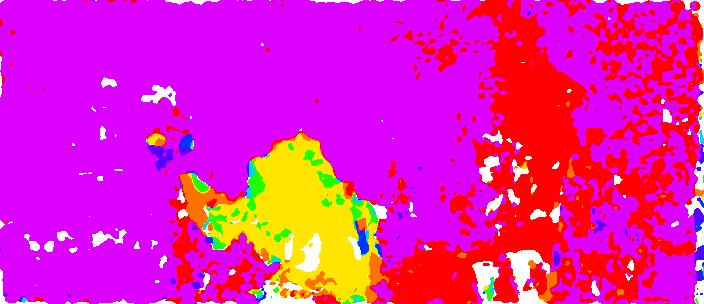
\includegraphics[width=.23\textwidth]{cvpr14_figures/flow/flow_actioncliptest00538_frame014_traj_quant.jpeg} \\
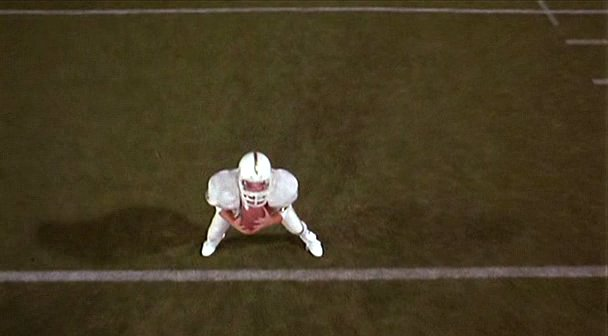
\includegraphics[width=.23\textwidth]{cvpr14_figures/flow/flow_actioncliptest00870_frame013.jpeg} & 

\includegraphics[width=.23\textwidth]{cvpr14_figures/flow/flow_actioncliptest00870_frame014_mv_quant.png} & 
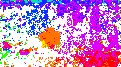
\includegraphics[width=.23\textwidth]{cvpr14_figures/flow/flow_actioncliptest00870_frame013_stip_quant.png} & 
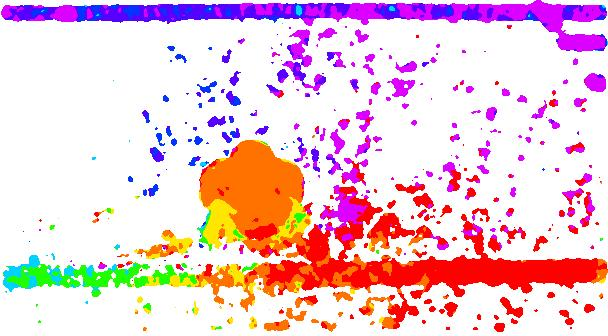
\includegraphics[width=.23\textwidth]{cvpr14_figures/flow/flow_actioncliptest00870_frame013_traj_quant.jpeg} \vspace{.2cm}\\
\end{tabular}
\caption[Qualitative comparison of optical flow]{Qualitative comparison of optical flow in real movie frames using flow estimation methods in Figure~\ref{fig:flow1}. All methods produce noisy flow estimates. Quantized values of MPEG flow are consistent with the quantized output of the two optical flow algorithms. We compare quantized flow values since these are used in descriptor computation by our and other methods.\vspace{-.3cm}}
\label{fig:flow2}
\end{center}
\end{figure*}



\subsection{Motion fields from video compression}
Consequent video frames are highly redundant with most of the changes between frames typically originating from the object or camera motion. As the storage of sparse motion vectors is much more efficient compared the storage of pixel values, video compression schemes heavily rely on motion estimation and encode coarse motion information in compressed video representations such as MPEG. This motion field can be accessed at the time of video decompression without additional cost\footnote{Full video decompression may not be required.}. %to access motion information. We currently perform full video decompression due to implementation reasons, however, it could be changed, resulting in additional speed-up of our method in the future.}.

Motion estimation by video encoders is designed to optimize video compression size and may not necessarily correspond to the true motion in the video. To verify the quality of the motion field obtained from video compression (here called MPEG flow), we compare it with the ground truth flow as well as with the output of optical flow methods by Lucas and Kanade~\cite{Lucas81} and Farneb\"ack~\cite{Farneback03}. We choose these two methods since they are deployed in existing implementations of local motion descriptors~\cite{Laptev08} and~\cite{Wang12} which we use in this work for comparison. Figure~\ref{fig:flow1} illustrates the ground truth flow and automatic flow estimates obtained for a synthetic video sequence from the recent MPI Sintel dataset~\cite{Butler12}. For this experiment we quantize flow fields into eight orientation values and one ``no-motion'' bin since this representation of flow is used in this paper for the construction of our fast video descriptor. The details and measurement results are in Figure~\ref{fig:flow1}.

%difference in flow by comparing flow estimates with the ground truth using end point error (EPE), see Figure~\ref{fig:flow1}(left). In Figure~\ref{fig:flow1}(right) we show flow fields discretized into eight orientation bins and one ``no-motion'' bin\footnote{``No-motion'' bin represents motion vectors with the magnitude below $0.4$ pixels.}. Comparing consistency of this quantization is interesting as we use it later for constructing histogram-based local motion descriptors. 

We have evaluated quantitative performance of MPEG flow in the standard Clean setup of the MPI Sintel benchmark. Despite the fact that the motion field obtained from MPEG flow has low resolution, the obtained results (EPE all=11.148 and EPE matched=6.706) outperform several methods reported on the MPI Sintel web-page {\small \url{http://sintel.is.tue.mpg.de/results}}. Qualitatively, the level of noise in MPEG flow and optical flow estimates is comparable both for synthetic and real video examples as illustrated in Figure~\ref{fig:flow2}. This indicates that the substitute of the slow optical flow used in video descriptors~\cite{Laptev08,Wang12} by the ``virtually free'' MPEG flow may not have large implications on the performance of subsequent recognition steps.


%094fad32-4801-11e1-8d64-f0def1b7a4f4



%MPEG flow
%overall EPE error 4.559; overall mag 4.981
%overall quantization error 0.196 (5bins); quantization error 0.283 (9bins)
%
%LK flow (in STIP)
%overall EPE error 4.949; overall mag 5.344
%overall quantization error 0.256 (5bis); quantization error 0.334 (9bins)
%
%DT flow
%overall EPE error 3.192; overall mag 5.334
%overall quantization error 0.214 (5bins); quantization error 0.286 (9bins)




\subsection{MPEG flow video descriptor}
\label{sec:CDdescriptor}

We follow the design of previously proposed local space-time descriptors~\cite{Laptev08,Wang12} and define our descriptor by histograms of MPEG flow vectors accumulated in a video patch. Each patch is divided into cells as illustrated in Figure~\ref{fig:CDdescriptor} and the normalized histograms from patch cells are concatenated into a descriptor vector. Constrained by the coarse $16\times16$ pixel spatial resolution of MPEG flow, we align descriptor grid cells with positions of motion vectors (red points in Figure~\ref{fig:CDdescriptor}). We also use bilinear interpolation of flow and increase the spatial resolution of the flow field by the factor of two (yellow points in Figure~\ref{fig:CDdescriptor})\footnote{We found interpolation of the flow to be important in our experiments}. 

Following~\cite{Wang12}, we compute HOF descriptors as histograms of MPEG flow discretized into eight orientation bins and a no-motion bin. For MBHx and MBHy descriptors the spatial gradients of the $v_x$ and $v_y$ components of the flow are similarly discretized into nine orientation bins. %We compute HOF, MBHx, MBHy histograms by accumulating quantized flow values within each cell (see Figure~\ref{fig:CDdescriptor}). 
The final descriptor is obtained by concatenating histograms from each cell of the $2\times2\times3$ descriptor grid followed by $l_2$-normalization of every temporal slice. HOG descriptors are computed at the same sparse set of points.

The above scheme defines a $32\times32\times15$ pixel descriptor which we compute at every location of the video defined by the spatial stride of $16$ pixels and temporal stride of $5$ frames. To sample multiple spatial scales, we similarly define a $48\times48\times15$ pixel descriptor sampled with $24$ pixels spatial stride. For a video of $640\times480$ pixels spatial resolution we obtain around 300 descriptors per frame. This is comparable to $\approx350$ dense trajectory features produced by the method in~\cite{Wang12} for the same video resolution.

Main computational advantages of our descriptor originate from the elimination of the optical flow computation and from the coarse sampling of flow vectors. As we demonstrate experimentally in Section~\ref{sec:experiments}, these modifications imply drastic improvements of computational requirements at the cost of minor reduction in the classification performance. 


\begin{figure}
\begin{center}
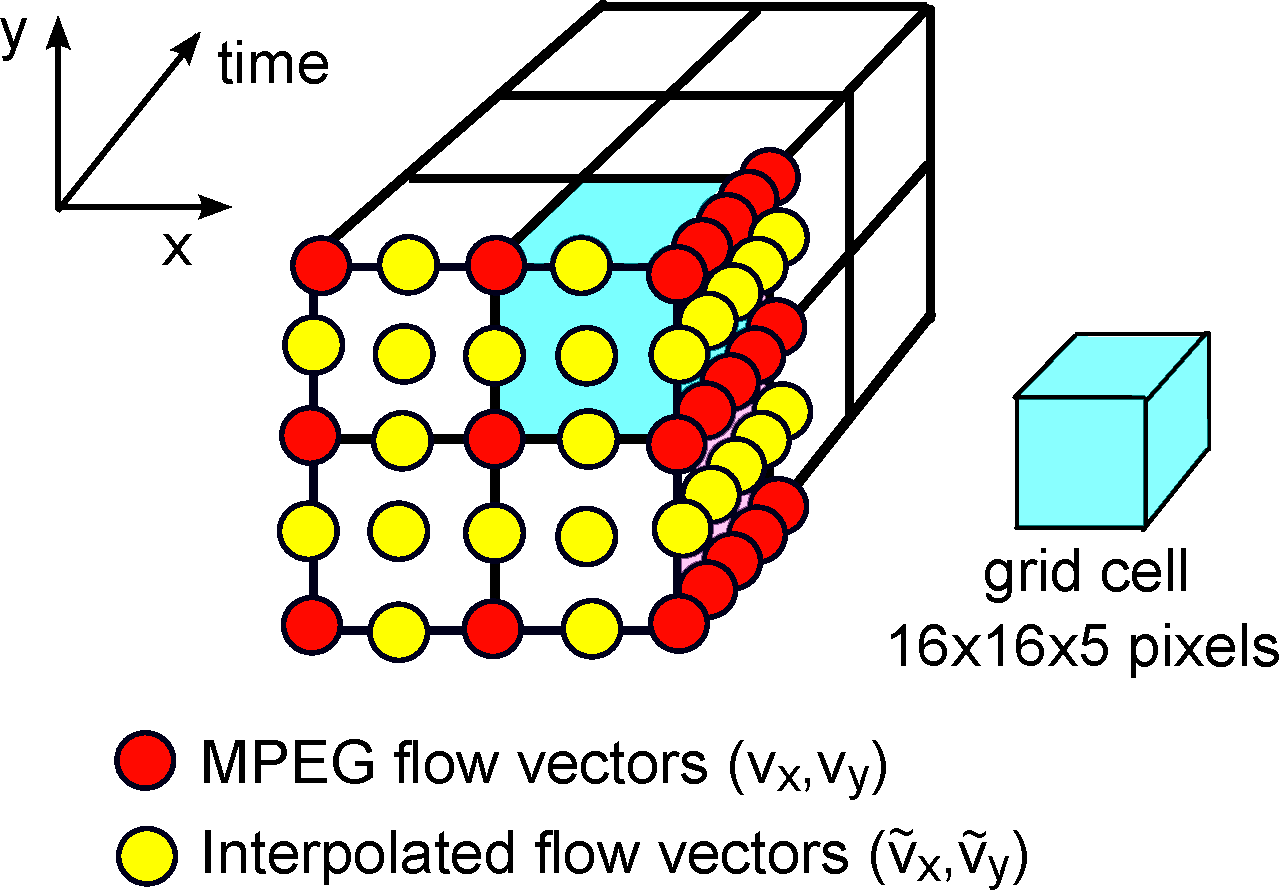
\includegraphics[width=.6\linewidth]{cvpr14_figures/CD-descriptor2.pdf}
\caption[MPEG flow video descriptor]{MPEG flow (MF) video descriptor defined at positions of MPEG flow vectors. Each $2\times2\times3$ descriptor cell is accumulated from quantized values of original and interpolated flow vectors indicated by the red and yellow circles respectively.\vspace{-.6cm}}
\label{fig:CDdescriptor}
\end{center}
\end{figure}


\begin{figure*}[!t]
\begin{center}
\vspace{-.6cm}
%\begin{tabular}{cccccc}
%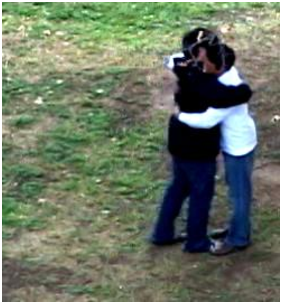
\includegraphics[scale=0.2]{cvpr14_figures/dataset_thumb/uti/crop_class1.pdf} & 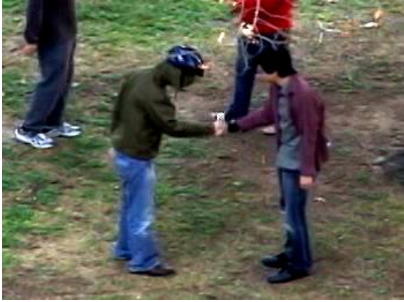
\includegraphics[scale=0.2]{cvpr14_figures/dataset_thumb/uti/crop_class2.pdf} & 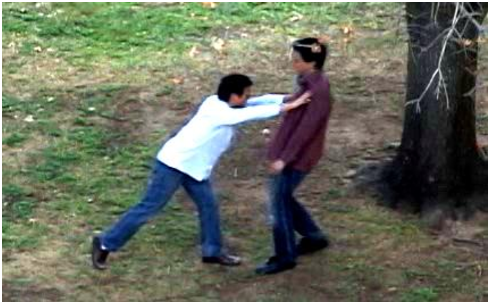
\includegraphics[scale=0.2]{cvpr14_figures/dataset_thumb/uti/crop_class3.pdf} & 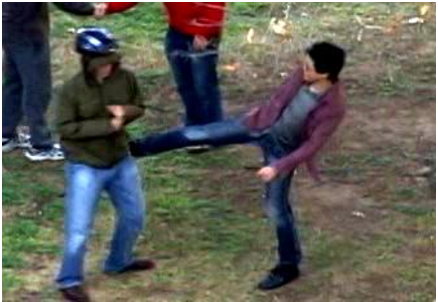
\includegraphics[scale=0.2]{cvpr14_figures/dataset_thumb/uti/crop_class4.pdf} & 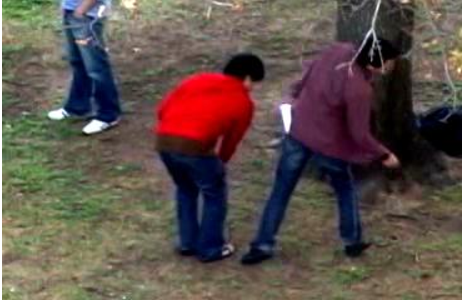
\includegraphics[scale=0.2]{cvpr14_figures/dataset_thumb/uti/crop_class5.pdf} & 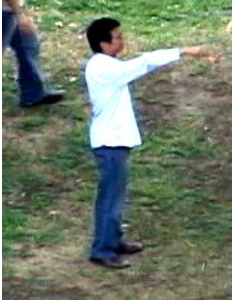
\includegraphics[scale=0.2]{cvpr14_figures/dataset_thumb/uti/crop_class6.pdf} \\
%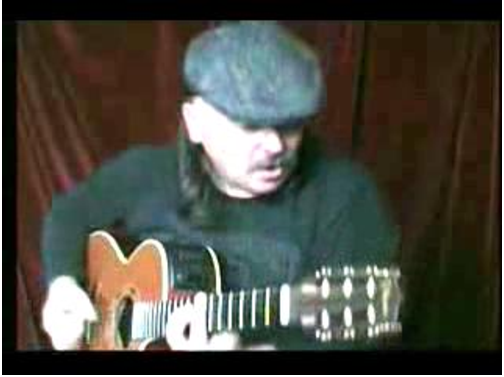
\includegraphics[scale=0.2]{cvpr14_figures/dataset_thumb/ucf/crop_class1.pdf} & 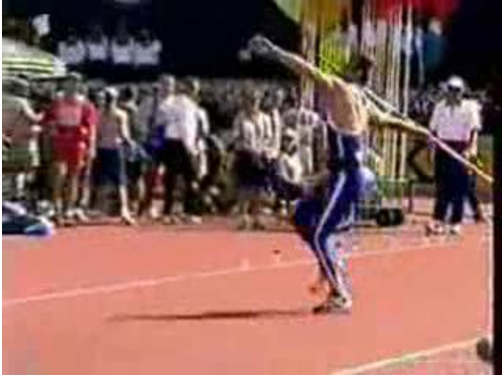
\includegraphics[scale=0.2]{cvpr14_figures/dataset_thumb/ucf/crop_class2.pdf} & 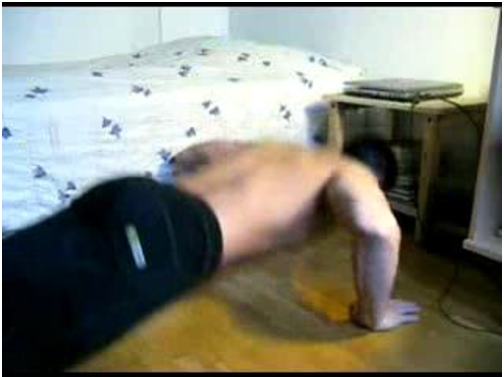
\includegraphics[scale=0.2]{cvpr14_figures/dataset_thumb/ucf/crop_class3.pdf} & 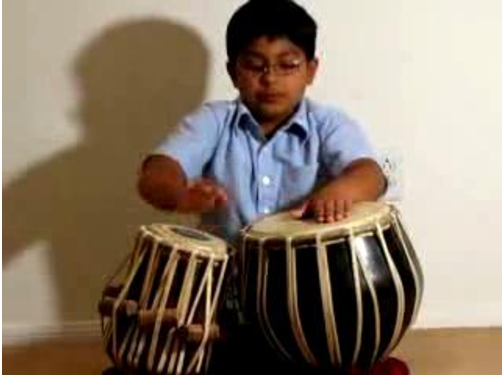
\includegraphics[scale=0.2]{cvpr14_figures/dataset_thumb/ucf/crop_class4.pdf} & 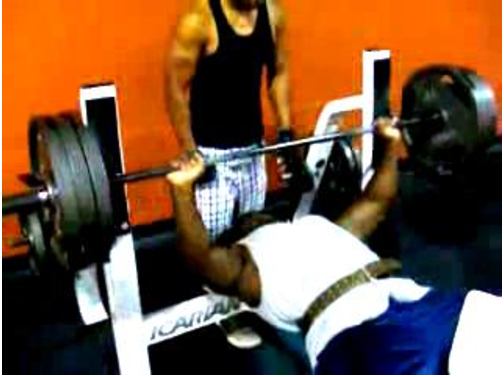
\includegraphics[scale=0.2]{cvpr14_figures/dataset_thumb/ucf/crop_class5.pdf} & 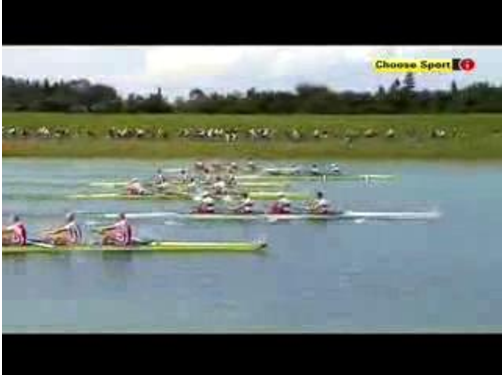
\includegraphics[scale=0.2]{cvpr14_figures/dataset_thumb/ucf/crop_class6.pdf} \\
%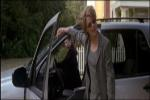
\includegraphics[height=1cm]{cvpr14_figures/dataset_thumb/hwd/class1.jpg} & 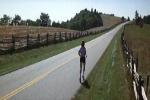
\includegraphics[height=1cm]{cvpr14_figures/dataset_thumb/hwd/class2.jpg} & 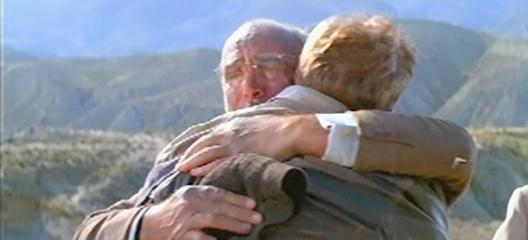
\includegraphics[height=1cm]{cvpr14_figures/dataset_thumb/hwd/class3.jpg} & 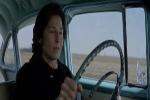
\includegraphics[height=1cm]{cvpr14_figures/dataset_thumb/hwd/class4.jpg} & 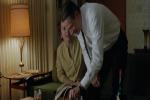
\includegraphics[height=1cm]{cvpr14_figures/dataset_thumb/hwd/class5.jpg} & 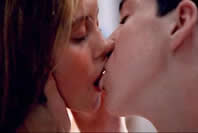
\includegraphics[height=1cm]{cvpr14_figures/dataset_thumb/hwd/class6.jpg} \\
%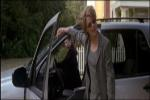
\includegraphics[height=1.61cm]{cvpr14_figures/dataset_thumb/hwd/class1.jpg} 
%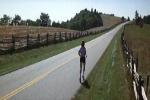
\includegraphics[height=1.61cm]{cvpr14_figures/dataset_thumb/hwd/class2.jpg} 
%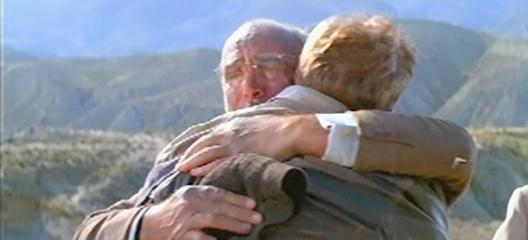
\includegraphics[height=1.61cm]{cvpr14_figures/dataset_thumb/hwd/class3.jpg}  
%\includegraphics[height=1.61cm]{cvpr14_figures/dataset_thumb/hwd/class4.jpg}
%\includegraphics[height=1.61cm]{cvpr14_figures/dataset_thumb/hwd/class5.jpg}
%\includegraphics[height=1.61cm]{cvpr14_figures/dataset_thumb/hwd/class6.jpg} \\
%\includegraphics[scale=0.305]{cvpr14_figures/dataset_thumb/ucf/crop_class1.pdf}
%\includegraphics[scale=0.305]{cvpr14_figures/dataset_thumb/ucf/crop_class2.pdf}
%\includegraphics[scale=0.305]{cvpr14_figures/dataset_thumb/ucf/crop_class3.pdf} 
%\includegraphics[scale=0.305]{cvpr14_figures/dataset_thumb/ucf/crop_class4.pdf} 
%\includegraphics[scale=0.305]{cvpr14_figures/dataset_thumb/ucf/crop_class5.pdf} 
%\includegraphics[scale=0.305]{cvpr14_figures/dataset_thumb/ucf/crop_class6.pdf} \\
%\includegraphics[scale=0.4]{cvpr14_figures/dataset_thumb/uti/crop_class1.pdf} 
%\includegraphics[scale=0.4]{cvpr14_figures/dataset_thumb/uti/crop_class2.pdf} 
%\includegraphics[scale=0.4]{cvpr14_figures/dataset_thumb/uti/crop_class3.pdf} 
%\includegraphics[scale=0.4]{cvpr14_figures/dataset_thumb/uti/crop_class4.pdf} 
%\includegraphics[scale=0.4]{cvpr14_figures/dataset_thumb/uti/crop_class5.pdf} 
%\includegraphics[scale=0.4]{cvpr14_figures/dataset_thumb/uti/crop_class6.pdf} \\
\includegraphics[height=1.3cm]{cvpr14_figures/dataset_thumb/hwd/class1.jpg} 
\includegraphics[height=1.3cm]{cvpr14_figures/dataset_thumb/hwd/class2.jpg} 
\includegraphics[height=1.3cm]{cvpr14_figures/dataset_thumb/hwd/class3.jpg}  
\includegraphics[height=1.3cm]{cvpr14_figures/dataset_thumb/hwd/class4.jpg}
\includegraphics[height=1.3cm]{cvpr14_figures/dataset_thumb/hwd/class5.jpg}
\includegraphics[height=1.3cm]{cvpr14_figures/dataset_thumb/hwd/class6.jpg} \\
\includegraphics[scale=0.25]{cvpr14_figures/dataset_thumb/ucf/crop_class1.pdf}
\includegraphics[scale=0.25]{cvpr14_figures/dataset_thumb/ucf/crop_class2.pdf}
\includegraphics[scale=0.25]{cvpr14_figures/dataset_thumb/ucf/crop_class3.pdf} 
\includegraphics[scale=0.25]{cvpr14_figures/dataset_thumb/ucf/crop_class4.pdf} 
\includegraphics[scale=0.25]{cvpr14_figures/dataset_thumb/ucf/crop_class5.pdf} 
\includegraphics[scale=0.25]{cvpr14_figures/dataset_thumb/ucf/crop_class6.pdf} \\
\includegraphics[scale=0.19]{cvpr14_figures/dataset_thumb/hmdb/class1.png}
\includegraphics[scale=0.19]{cvpr14_figures/dataset_thumb/hmdb/class2.png}
\includegraphics[scale=0.19]{cvpr14_figures/dataset_thumb/hmdb/class3.png} 
\includegraphics[scale=0.19]{cvpr14_figures/dataset_thumb/hmdb/class4.png} 
\includegraphics[scale=0.19]{cvpr14_figures/dataset_thumb/hmdb/class5.png} 
\includegraphics[scale=0.19]{cvpr14_figures/dataset_thumb/hmdb/class6.png} \\
\includegraphics[scale=0.32]{cvpr14_figures/dataset_thumb/uti/crop_class1.pdf} 
\includegraphics[scale=0.32]{cvpr14_figures/dataset_thumb/uti/crop_class2.pdf} 
\includegraphics[scale=0.32]{cvpr14_figures/dataset_thumb/uti/crop_class3.pdf} 
\includegraphics[scale=0.32]{cvpr14_figures/dataset_thumb/uti/crop_class4.pdf} 
\includegraphics[scale=0.32]{cvpr14_figures/dataset_thumb/uti/crop_class5.pdf} 
\includegraphics[scale=0.32]{cvpr14_figures/dataset_thumb/uti/crop_class6.pdf} \\
%\end{tabular}
\smallskip
\caption[Sample frames from action recognition datasets]{Sample frames from action recognition datasets. From top to bottom: Hollywood2~\cite{Marszalek09}, UCF50~\cite{Reddy12}, HMDB51~\cite{Kuehne11}, UT-Interaction~\cite{Ryoo10}.\vspace{-.5cm}}
\label{fig:datasets}
\end{center}
\end{figure*}




\section{Experimental evaluation}\label{sec:experiments}
%%%%%%%%%%%%%%%%%%%%%%%%%%%%%%%%%%%%%%%%%%%%%%%%%%%%%%%%%%%%%%%%
%%%%%%%%%%%%% Experimental evaluation
%%%%%%%%%%%%%%%%%%%%%%%%%%%%%%%%%%%%%%%%%%%%%%%%%%%%%%%%%%%%%%%%
\begin{table*}[t!]
\begin{center}
\begin{tabular}{p{.65\textwidth}p{.32\textwidth}}
\hspace*{.4cm}
\begin{tabular}{|l||c|c||c|c|}
\hline
\multirow{3}{*}{} &\multicolumn{2}{c||}{Classification} & \multicolumn{2}{c|}{Speed}\\
                  &\multicolumn{2}{c||}{(mAP)} & \multicolumn{2}{c|}{(fps)}\\
\cline{2-5}
& MF (our) & DT~\cite{Wang12} & MF (our) & DT~\cite{Wang12}\\
\hline\hline
HOF               & 47.2\% & 52.9\% & 346.8 &  \\\hline
MBHx              & 49.0\% & 52.0\% & 330.3 &  \\\hline
MBHy              & 50.4\% & 56.1\% & 330.3 &  \\\hline
HOF+MBHx+MBHy     & 53.9\% & 58.9\% & 218.7 &  \\\hline
HOF+MBHx+MBHy+HOG & 56.2\% & 60.0\% & 168.4 & 1.2 \\\hline
\end{tabular}
&
\mbox{}\vspace{-.55cm}\newline
\hspace*{.2cm}
\begin{tabular}{|l|c|c|}
\hline
             & xvid  & x264  \\\hline
5000 kbit/s  & 58.9\% & 57.5\% \\\hline
1000 kbit/s   & 58.2\% & 57.4\% \\\hline
500 kbit/s   & 57.7\% & 57.1\% \\\hline
250 kbit/s   & 57.7\% & 57.0\% \\\hline
\end{tabular}
%

\end{tabular}
\mbox{}\vspace{.1cm}\\
\caption[Evaluation of action classification accuracy]{{\bf Left:} Evaluation of action classification accuracy and the speed of feature computation for Hollywood2 action recognition benchmark. The speed of feature computation is reported for video of spatial resolution $640\times480$ pixels. {\bf Right:} Evaluation of action recognition accuracy in Hollywood2 under the variation of video compression in terms of video codecs and compression bit-rates. The results are reported for MF descriptors in combination with FV encoding.\vspace{-.2cm}}
\label{tab:HWD2}
\end{center}
\end{table*}

%In this section we evaluate the proposed descriptor and descriptor encoding schemes on Hollywood2~\cite{Marszalek09} and UCF50~\cite{Reddy12} action recognition benchmarks and compare the speed and the recognition accuracy to the state of the art. We report classification results as mean average precision (mAP) for Hollywood2 and accuracy (Acc.) for UCF50. Processing speed is reported as frame-per-second (fps). We first evaluate the accuracy and the computational cost of proposed descriptor and compare it to the state-of-the-art method~\cite{Wang11}. The second part of the evaluation concerns the speed and accuracy of descriptor encoding.

In this section we evaluate the proposed descriptor and encoding schemes on Hollywood2~\cite{Marszalek09}, UCF50~\cite{Reddy12}, HMDB51~\cite{Kuehne11} and UT-Interaction~\cite{Ryoo10} action recognition benchmarks (see Figure~\ref{fig:datasets}) and compare the speed and accuracy of action recognition to recent methods~\cite{Feng13,Wang12,Yu10}. We follow standard evaluation setups and report mean average precision (mAP) for Hollywood2 and mean accuracy (acc) for UCF50, HMDB51 and UT-Interaction datasets. The processing speed is reported in frames-per-second (fps), run at a single-core Intel Xeon E5345 (2.33 GHz).

%In this series of experiments we adopt the standard bag-of-features action classification pipeline~\cite{Schuldt04} and represent each video clip by a $l_1$-normalized histogram of quantized local features. For each extracted type of descriptor we compute a vocabulary of 4000 visual words using k-means and assign all features to their nearest visual word centroids. Taking into account the space-time pyramid, we end up with $4\times24=96$ channels which we put in the SVM with multi-channel exponential $\chi^2$-kernel~\cite{Zhang07}.

To recognize actions we use SVM with multi-channel exponential $\chi^2$-kernel~\cite{Zhang07} together with histogram-based action representations. For Fisher vector and VLAD encodings we use linear SVMs.


\subsection{Descriptor evaluation}
%To assess the performance of motion information in compressed video representation, we first evaluate the performance of STIP features~\cite{Laptev08} where MPEG flow was obtained from DivX compression of Hollywood2 video samples and upscaled to the original video resolution. Results for one channel HOF descriptors in this setup gives 0.432 mAP compared to 0.458 mAP obtained for the original STIP implementation using Lucas-Kanade optical flow.

Table~\ref{tab:HWD2}~(Left) presents results of action recognition using the proposed MPEG flow (MF) features %described in Section~\ref{sec:CDdescriptor} 
compared to Dense Trajectories (DT) baseline~\cite{Wang12} using histogram encoding. For the full combination of four descriptors the performance of DT ($\sim$60.0\%) is approximately four per-cent higher compared to MF features ($\sim$56.2\%). When comparing the speed of feature extraction for both methods measured on videos with $640\times480$ pixels spatial resolution, our method achieves 168fps which is about 7 times faster than real-time and 140 times faster compared to~\cite{Wang12}. The speed measurements in this experiment include the time of feature computation as well as the time for video reading and decompression. Our method spends most of the time on the aggregation of histogram-based video descriptors using intergral space-time histograms. 
Compared to~\cite{Wang12} we save $\sim$66\% by avoiding OF computation, $\sim$4\% by sparser descriptor sampling and $\sim$29\% by the aggregation of sparse motion vectors. The run-time of our descriptor is, hence, $<$1\% of descriptor computation time in~\cite{Wang12}. Reducing the number of descriptor types increases the speed of our method to 347fps (14 times real time) at the cost of $<$4\% drop in mAP. 

DT features~\cite{Wang12} are computed along point tracks which is different to our features computed inside the fixed-size video patches. To identify the source of $\sim$4\% mAP drop of our method compared to~\cite{Wang12}, we simplify DT features by first approximating free-shape trajectories in DT features by constant velocity trajectories (DT V*). In the second simplification we remove trajectory information from DT descriptor and compute DT features in fixed axes-parallel cuboids (DT V0). The results of these modifications in the first two lines of Table~\ref{tab:HWD2traj} indicate 1\% drop due to DT V* and 1\% further drop in mAP due to DT V0. Explicitly including the shape of trajectories into the descriptor (last line of Table~\ref{tab:HWD2traj}) does not improve performance significantly. From this experiment we conclude that the shape of trajectories does not contribute to other descriptors significantly. We believe that the difference in accuracy of DT features and our method should be in the denser and more accurate flow estimation deployed by DT. Per-class action classification comparison of MF and DT features is illustrated in Figure~\ref{fig:hwd2-barplot}.

\begin{table}
\begin{center}
\begin{tabular}{|l|c|c|}
\hline
& mAP \\\hline
HOF+MBHx+MBHy+HOG (V0)  					& 58.0\%	\\\hline
HOF+MBHx+MBHy+HOG (V*)						& 58.9\%	\\\hline
HOF+MBHx+MBHy+HOG \cite{Wang12}     	& 60.0\% 	\\\hline
HOF+MBHX+MBHY+HOG+TRAJ \cite{Wang12} 	& 60.3\% 	\\\hline
\end{tabular}
\mbox{}\vspace{.2cm}\\
\caption[Action classification accuracy]{Action classification accuracy on Hollywood2 dataset for different versions of the dense trajectory features~\cite{Wang12} in combination with histogram encoding}
\label{tab:HWD2traj}
\end{center}
\end{table}



\subsection{Descriptor encoding evaluation}
\label{subsec:descencimprov}
While our method achieves high speed descriptor computation, the feature quantization becomes a bottle-neck with nearest-neighbor (NN) quantization performing only at the rate of 10fps when using efficient $l_2$-distance implementation. To improve quantization speed, we experiment with tree-based approximate nearest neighbor (ANN) quantization schemes implemented in FLANN~\cite{Muja09}. The trade-off between computational time and the accuracy of quantization measured on the final recognition task is illustrated in Figure~\ref{fig:hwd2-flann}. Notably, the quantization using four trees and 32 tests in ANN search does not degrade recognition performance and achieves factor $\approx$ 5x speed-up compared to NN. Further increase of the speed implies approximately linear degradation of classification accuracy. 

We next investigated Fisher Vector (FV)~\cite{Perronnin12} and VLAD encodings~\cite{Jegou10} described in Section~\ref{sec:quantization}. 
%FV and VLAD representations have been shown to achieve high accuracy for image classification tasks~\cite{Chatfield11} and usually require smaller vocabularies compared to histogram encodings.
%
%Fisher vector and VLAD schemes are described in Section~\ref{sec:quantization}. 
The VLAD encoding has already been applied to action reconition in \cite{Jain13}, but here we also evaluate the full Fisher vector. We train a GMM model with $K=256$ Gaussians \cite{Jegou12}. Results in Figure~\ref{fig:hwd2-flann} and Table~\ref{tab:hwd2_comparison} indicate improvements in both the speed and accuracy when using FV and VLAD encodings compared to the histogram encoding. As for the histogram encoding, FLANN provides considerable speed-up for FV and VLAD encodings.

Table~\ref{tab:ucf_comparison} presents action recognition results for the UCF50 dataset. Similar to the Hollywood2 dataset, the accuracy of our methods is only a few percent below the state-of-the-art results in~\cite{Wang12} with FV and VLAD encodings providing improvements over the histogram encoding both in speed and accuracy. The overall speed improves the speed of~\cite{Wang12} by two orders of magnitude. Table~\ref{tab:uti_comparison} presents results for the UT-Interaction dataset and compares our method with the efficient action recognition method~\cite{Yu10}. Our method demonstrates better classification accuracy compared to~\cite{Yu10} and improves the speed of~\cite{Yu10} by one order of magnitude. %the factor of $10$.

In Table~\ref{tab:hmdb_comparison} we compare our results on the HMDB dataset to~\cite{Feng13} that investigates the effect of feature sampling on the trade-off between computational efficiency and recognition performance. For the MBH descriptor our method obtains significant improvement both in speed and accuracy, despite the fact that in~\cite{Feng13} the system was evaluated on Intel i7-3770K (3.50 GHz) which runs 1GHz faster than our Intel Xeon E5345 (2.33 GHz). Both systems were evaluated on a single core with no multithreading.

%Our Fisher vector implementation attributes a descriptor only to 5 nearest mixture centroids in $l_2$-sense in contrast to \cite{Jegou12} which fully computes $q_{ki}$ to all mixture centroids in their public implementation in the YAEL library\footnote{\scriptsize \url{https://gforge.inria.fr/projects/yael/}}. To make it faster we compute only the 5 nearest neighbors using kd-trees. Differently from YAEL we explicitly tailor our implementation to efficiently compute Fisher vector for several spatio-temporal grids. In addition, we found that the second order part $\textbf{v}_k$ (\ref{eq:fv_vk}) does not bring improvement, and we don't compute it.

%We also experiment with the VLAD representation that we get if we consider only one nearest neighbor during the process described above. With both representations we try different values for the number of tests performed during the descent down the kd-trees.

Recently, the method in \cite{Wang12} has been further improved using motion stabilization~\cite{Jain13,Wang13} and feature extraction from person tracks~\cite{Wang13}. These extensions are complementary to our work and can be used to improve results of our method.
%The authors also use Fisher vectors but without space-time binning. The accuracy is significantly higher than in \cite{Wang12} ($64.3\%$ on Hollywood2, $57.2\%$ on HMDB51 and $91.2\%$ for UCF50), but the speed is roughly the same. We consider the lower sparsity of optical flow and low number of descriptors per frame to be the main source of decreased accuracy of our method (see Table~\ref{tab:HWD2traj} (V0) compared to Table~\ref{tab:HWD2}). However, in need of very efficient action recognition the trade-off may be worth it. We consider the extensions of~\cite{Wang13} may be implemented in our method as well, but the efficiency will need to be studied.


\begin{table}
\begin{center}
\vspace{-.1cm}
\begin{tabular}{r|c|c|c|c|}
\cline{2-5}
& \multicolumn{2}{c|}{Farneback flow} & \multicolumn{2}{c|}{MPEG flow} \\\hline
\multicolumn{1}{|r|}{Sampling stride} & mAP & fps & mAP & fps \\\hline
\multicolumn{1}{|r|}{16}  	& 58.3\% & 35.2	& 58.2\% & 168.4\\\hline
\multicolumn{1}{|r|}{8}   	& 58.6\% & 24.1 & &	\\\hline
\multicolumn{1}{|r|}{4}     	& 59.2\% & 13.7	& &     \\\hline
\end{tabular}
\mbox{}\vspace{.2cm}\\
\caption[Action classification accuracy on Hollywood2 dataset]{Action classification accuracy on Hollywood2 dataset using sparse sampling of Farneback flow and MPEG flow followed by FV feature encoding. The reported speed of feature extraction is affected by the increased computational cost of aggregating motion vectors into local descriptors. \vspace{-.6cm}}
\label{tab:flow_resample}
\end{center}
\end{table}



\subsection{Parameter sensitivity}
MPEG flow might be influenced by the types and parameters of video codecs. To investigate this aspect, we evaluate the performance of action recognition for two common video codecs (x264 and xvid) under varying video compression bit-rates. Results in Table~\ref{tab:HWD2} (Right) indicate the stable performance of action recognition for different types of video codecs and decreasing video quality corresponding to low values of bit-rates. 

We have also evaluated the influence of sparse flow sampling on the speed and accuracy of action recognition. In Table~\ref{tab:flow_resample} we illustrate accuracy of our method when using Farneback flow and MPEG flow. Denser flow sampling (Farneback) leads to slight improvements in recognition accuracy by the cost of significantly increased computation time. Notably, sparse Farneback and MPEG flow show similar recognition performance.

\begin{figure}
\begin{center}
\includegraphics[width=.9\linewidth]{cvpr14_figures/hollywood2-per-class-barplot-crop.pdf}.
\caption[Per-class action classification results]{Per-class action classification results for DT~\cite{Wang12} and our  MF features using HOF+MBHx+MBHy+HOG descriptor combination and histogram encoding on the Hollywood2 benchmark.\vspace{-.1cm}}
\label{fig:hwd2-barplot}
\end{center}
\end{figure}

\begin{figure}
\begin{center}
\mbox{}\vspace{-.4cm}\\
\includegraphics[width=.9\linewidth]{cvpr14_figures/hollywood2-flann-fps-map-crop-mod.pdf}
\caption[Performance of action recognition]{Performance of action recognition and the speed of descriptor encodings in Hollywood2 dataset for different types and parameters of encoding schemes. kd($x$) indicates the number of trees $x$ in the kd-forest used for ANN descriptor assignment. ch($y$) indicates the number of tests $y$ when descending the forest.\vspace{-.4cm}}
\label{fig:hwd2-flann}
\end{center}
\end{figure}




\begin{table}
\begin{center}
\begin{tabular}{|l|c|c|c|c|}
\hline
		 				&  	 		& Feat.                   	& Quant. 		& Total		\\
		 				& Acc.  	& (fps)								& (fps)			& (fps)		\\\hline
MF FLANN(4-32)	& 55.8\%	& \multirow{3}{*}{168.4} 	& 52.4    	& 40.0 	\\ % FPS = 1/(1/168.4 + 1/52.3921)
MF VLAD(4) 		& 56.7\%	&										& 167.5	& 84.0	\\ % FPS = 1/(1/168.4 + 1/167.537313)
MF FV(32)			& 58.2\%	&										& 40.9 	& 32.9	\\ % FPS = 1/(1/168.4 + 1/40.8925322)
\hline
DT \cite{Wang12}& 59.9\%		& 1.2									& 5.1 		&	1.0	\\\hline % Quant. FPS = 1346 frames / 266.17 secs = 5.0569 FPS; Total = 1/(1/1.2 + 1/5.0569) = 0.9699 FPS
%\cite{le_at_al}						& 53.3\%		&										&				&\\\hline
\end{tabular}
\mbox{}\\
\caption[Comparison of our method to the state of the art on Hollywood2 dataset]{Comparison of our method to the state of the art on Hollywood2 dataset. The speed of~\cite{Wang12} and of our method is reported for videos with spatial resolution $640\times 480$ pixels.\vspace{-.3cm}}
\label{tab:hwd2_comparison}
\end{center}
\end{table}



\begin{table}
\begin{center}
\begin{tabular}{|l|c|c|c|c|}
\hline
		 				&  	 	& Feat.                    & Quant. 	& Total	\\
		 				& Acc.  & (fps)                    & (fps) 	& (fps)	\\\hline
MF FLANN(4-32)	& 81.6\% & \multirow{3}{*}{591.8}   & 52.4  	& 48.1	\\ % FPS = 1/(1/592 + 1/52.3921)
MF VLAD(4) 	 	& 80.6\% &                          & 671.4 	& 314.6	\\ % FPS = 1/(1/592 + 1/671.428571)
MF FV(32)	 		& 82.2\% &                          & 171.3 	& 132.8	\\ % FPS = 1/(1/592 + 1/171.255061)
\hline
DT \cite{Wang12}& 85.6\% & 2.8            	        & 5.1  	& 1.8\\\hline%  Feat extr FPS = 846 frames / 5m; Quant FPS = 846 frames / 166.17 secs = 5.0912 FPS; Total = 1 / (1/2.8 + 1/5.0912) = 1.8065 FPS
%\cite{Kliper12}		&	72.7\%	&									&			&\\\hline
\end{tabular}
\smallskip
\caption[Comparison of our method to the state of the art on the UCF50 dataset]{Comparison of our method to the state of the art on the UCF50 dataset~\cite{Reddy12}. The speed is reported for videos with the spatial resolution $320\times 240$ pixels.}
\label{tab:ucf_comparison}
\mbox{}\vspace{-1cm}\\
\end{center}
\end{table}


\begin{table}
\begin{center}
\begin{tabular}{|l|c|c|}
% set1_segmented
%   sample acc = 85.238095
%   feat extr fps = 7280 frames / 15.990000 sec = 455.2846 fps
%	 quant time fps = 7280 frames / 61.720000 = 117.9520 fps
%   total_fps = 1 / (1/455.2846 + 1/117.9520) = 93.6816 fps
% set2_segmented
%	 sample acc = 87.6190
% 	 feat extr fps = 6515 frames / 12.160000 sec = 535.7730 fps
%   quant time fps = 6515 frames / 50.100000 = 130.0399fps
%   total_fps = 1 / (1/535.7730 + 1/130.0399) = 104.6418
% average fps: (93.6816 + 104.6418)/2 = 99.1617
% average acc: (85.238095 + 90.000000) / 2 = 87.6190
\hline
								& Acc.		& Total FPS	\\\hline
FV(32)						& 87.6\%		& 99.2		\\\hline
PSRM+BOST\cite{Yu10}	& 83.3\%		& 10.0 		\\\hline

\end{tabular}
\mbox{}\vspace{.2cm}\\
\caption[Accuracy and speed of action recognition]{Accuracy and speed of action recognition in the UT-interaction dataset~\cite{Ryoo10}.\vspace{-.6cm}}
\label{tab:uti_comparison}
\end{center}
\end{table}

\begin{table}
\begin{center}
\begin{tabular}{|l|c|c|c|c|}
\hline
% for KnifeThrowingJackDaggerDemoReel_throw_f_nm_np1_fr_med_2.avi (410 frames, 360x240)
		 				&  	 		& Feat.                    & Quant. 	& Total	\\
		 				& Acc.		& (fps)                    & (fps) 	& (fps)	\\\hline
MF ALL FV(32)		& 46.7\% 	& 455.6                    & 129.7 	& 101.0	\\ % FPS = 410 / 0.9 = 455.5556, 410 / 3.16 = 129.7468, 1 / (1/455.5556 + 1/129.7468) =   101.0
MF MBH FV(32)		& 45.4\% 	& 683.3                    & 268.0 	& 192.5	\\ % FPS = 410 / 0.6 = 683.3333, 410 / 1.53 = 267.9739, 1 / (1/683.3333 + 1/267.9739) =   192.4883
MF ALL VLAD(32) & 46.3\%	& 455.6								& 455.6		& 227.8	\\ % FPS = 410 / 0.9 = 455.5556, 1 / (1/455.5556 + 1/455.5556) =   227.7778
\hline
MBH \cite{Feng13}		& 41.1\% 	& 33.9            	     	& 267.1 & 30.8	\\ % FPS = 1/(1/41.19 + 1/192.4) = 33.9268
HOG3D \cite{Feng13}	& 33.3\% 	& 49.6            	   	& 290.8 & 42.2	\\ % FPS = 1/(1/71.88 + 1/159.60)= 49.5596
%Combined \cite{Feng13} & 47.6\% & 									&			&			\\
DT	\cite{Wang12}			& 48.3\%& 3.1								&			& \\ % FPS = 410 / 133.26 = 3.0767
\hline
\end{tabular}
\smallskip
\caption[Comparison of our method to \cite{Feng13} on the HMDB dataset~\cite{Kuehne11}]{Comparison of our method to \cite{Feng13} on the HMDB dataset~\cite{Kuehne11}. The speed is reported for videos with the spatial resolution $360\times 240$ pixels}
\label{tab:hmdb_comparison}
\mbox{}\vspace{-1cm}\\
\end{center}
\end{table}

%Hollywood2 results (A): Compressed domain features
%HOF: 0.472243
%MBHx: 0.490259
%MBHy: 0.503737
%HOF+MBHx+MBHy: 0.539212
%HOF+MBHx+MBHy+HOG (m/channel): 0.561959
%HOF+MBHx+MBHy+HOG (single vocab): 0.517230

%Hollywood2 results (B): Dense trajectory features
%HOF : 0.528732
%MBHX : 0.519922
%MBHY : 0.561268
%HOF_MBHX_MBHY : 0.589344
%HOF_MBHX_MBHY_HOG : 0.599716
%HOF_MBHX_MBHY_TRAJ : 0.591272
%HOF_MBHX_MBHY_HOG_TRAJ: 0.603235

%HOG+HOF+MBHx+MBHy:
%VEL0: 0.580140
%FST: 0.589389

%Hollywood2 results (C): Compressed domain features + FLANN; 
%HOF: 0.480621
%MBHx: 0.480726
%MBHy: 0.499320
%HOF+MBHx+MBHy: 0.540788
%HOF_MBHx_MBHy_HOG (m/channel): 0.564032

% per-class results in 
% https://docs.google.com/spreadsheet/ccc?key=0Al7q11u9-vugdDk4UlhrWjVxNm5Ldk9EMjVEZTZVM0E&pli=1#gid=0
% D:\doc\papers\descriptors\cvpr13\results\Class. results by class.xlsx

%%%%%%%%%%% computation time, election video 1800 frames 120 sec. 15fps (-> 72sec at 25fps)
% CD features   10.69 sec ->  168.3817 fps
% HOF only:     5.19 sec -> 346.8 fps
% MBHx 0nly:    5.45 sec -> 330.3 fps
% HOF+MBHx+MBHy 8.23 sec -> 218.7 fps
%
%# STAT. Descriptor computation: 3.13 secs
%# STAT. HOF: 0.42, MBH: 1.49 secs, HOG: 0.71 secs
%# STAT. Interpolation. HOFMBH: 0.14 secs, HOG: 0.37 secs
%# STAT. Descriptor querying: 3.60 secs
%# STAT. HOF: 0.84, MBH: 1.55 secs, HOG: 0.79 secs
%# STAT. Reading: 0.04 secs
%# STAT. Decoding: 3.75 secs
%# STAT. Writing: 87.96 secs
%# STAT. ---
%# STAT. Total: 98.65 secs
%# STAT. fps: 18.24
%# STAT. calls:
%# STAT. --ComputeDescriptor     6467808
%
% DT features: 24m56sec -> 1.2032 fps
%
% CD vs. DT speedup: x139.9449

%%%%%%%%%%% computation time, actioncliptest00775 1347 frames, 53.8 sec.
% CD features 9.35 sec -> 144.0642 fps
%# STAT. Descriptor computation: 2.79 secs
%# STAT. HOF: 0.29, MBH: 1.28 secs, HOG: 0.85 secs
%# STAT. Interpolation. HOFMBH: 0.07 secs, HOG: 0.30 secs
%# STAT. Descriptor querying: 3.22 secs
%# STAT. HOF: 1.00, MBH: 1.27 secs, HOG: 0.61 secs
%# STAT. Reading: 0.04 secs
%# STAT. Decoding: 3.00 secs
%# STAT. Writing: 71.45 secs
%# STAT. ---
%# STAT. Total: 80.80 secs
%# STAT. fps: 16.67
%# STAT. calls:
%# STAT. --ComputeDescriptor     4596504
%
% DT features 28m37sec -> 0.7845 fps
% real    28m37.449s
% user    28m26.158s
% sys     0m13.664s
%
% CD vs. DT speedup: x183.6382



% Quantization for actioncliptest00775 1347 frames, 53.8 sec.
%
%
% kd(8) + checks(32) 38.90 secs ->  34.6272      mAP 0.563959
% kd(8) + checks(16) 23.56 secs ->  57.1732      mAP 0.560811
% kd(8) + checks(8)  13.18 secs -> 102.2003      mAP 0.553482
% kd(8) + checks(4)  11.52 secs -> 116.9271      mAP 0.526568

% kd(4) + checks(32) 25.71 secs ->  52.3921 fps (mAP 0.564032)

% kd(4) + checks(16) 15.80 secs ->  85.2532     (mAP 0.557820)
% kd(4) + checks(8)  10.82 secs -> 124.4917     (mAP 0.552988)
% kd(4) + checks(4)   7.57 secs -> 177.9392     (mAP 0.542571)
% kd(2) + checks(32) 22.17 secs ->  60.7578     (mAP 0.552528)
% kd(2) + checks(16) 16.56 secs ->  81.3406     (mAP 0.556588)
% kd(2) + checks(8)  11.13 secs -> 121.0243     (mAP 0.549832)
% kd(2) + checks(4)   6.36 secs -> 211.7925     (mAP 0.538391)
%
%

%Quantization for actioncliptest00775 1347 frames, regular FV, just mu params
%Options:
%Indices are zero-based
%213-308 '../../vocab/mbhx_K256.vocab'
%Build GMM index: no
%GMM components: 256
%Lambda reg: 0.000000
%Output file path: out.npy
%Zero all gamma but: 0
%XnPos: 0, YnPos: 1, TnPos: 2
%Grids: 1x1x1x
%Vocabularies loaded
%
%#FV 1x1x1x  mbhx_K256 (213-308)
%fts.cols: 96
%24576
%No zeroing
%24576
%# 0-0-0 (380014)
%#STAT Vocab reading and construction: 0.03 secs
%#STAT Reading: 21.32 secs
%#STAT Writing: 0.00 secs
%#STAT Assigning: 164.76 secs
%#STAT Copying: 0.41 secs
%#STAT Total: 186.54 secs
%#STAT Ops: 1
%#STAT Descriptors: 380014
%#STAT Part sizes: 96

% Quantization for actioncliptest00775 w=640	h=480	frames=1347.00
%KNN_TREES_CHECKS FLANN ASSIGNING TOTAL FPS
%5_4_32 22.870000 10.070000 32.940000 40.892532		mAP 0.582075 (c =1e-3)
%5_4_16 13.890000 9.990000 23.880000 56.407035		mAP 0.571156 (c=1)
%5_4_8 9.000000 10.430000 19.430000 69.325785		mAP 0.566866 (c=1)
%5_4_4 6.720000 11.880000 18.600000 72.419355		mAP 0.558892 (c=1)

%1_4_32 19.780000 2.650000 22.430000 60.053500		mAP 0.567833 (c=1)
%1_4_16 11.580000 2.730000 14.310000 94.129979		mAP 0.563006 (c=0.1-1)
%1_4_8 7.540000 2.720000 10.260000 131.286550		mAP 0.561079 (c=1)
%1_4_4 5.300000 2.740000 8.040000 167.537313			mAP 0.553502 (c=1)

%3_4_32  21.350000       6.300000        27.650000       48.716094 mAP 0.565615 (c=1)
%3_4_16 mAP 0.562545 (c=1e-1)
%3_4_8 mAP 0.565996 (c=1)
%3_4_4   5.730000        6.760000        12.490000       107.846277 mAP 0.558180 (c=1)



%UCF50 w=320	h=240 frames=846.00 v_Rowing_g15_c05.avi  ; #features: 48944 => 57.8 features / frame
%5_4_32  3.350000        1.590000        4.940000        171.255061
%1_4_4   0.810000        0.450000        1.260000        671.428571
% feature extraction:  1.4200 => 595.7746 fps
%5_4_32 => total fps: 132.8761
%1_4_4  => total fps: 315.6401


%HMDB51 w=320 h=240	frames=75.0 Iaido_video_instruction_series_Wehrhahn_Sensei_sword_exercise_f_nm_np1_le_bad_1.avi  ; #features: 3864 => 51.5 features / frame
%5_4_32  0.300000        0.110000        0.410000        182.926829
%1_4_4   0.060000        0.040000        0.100000        750.000000
% feature extraction: 0.18sec => 416.6667 fps
%5_4_32 => total fps: 127.0918
%1_4_4  => total fps: 267.5815

%UCF50 extr. time on v_Rowing_g15_c05.avi. !! DescrComp + Interp + DescrQue + Reading + Decoding: 1.43 sec, 846 frames => 592 fps 
%# STAT. Descriptor computation: 0.47 secs
%# STAT. HOF: 0.05, MBH: 0.21 secs, HOG: 0.15 secs
%# STAT. Interpolation. HOFMBH: 0.01 secs, HOG: 0.05 secs
%# STAT. Descriptor querying: 0.55 secs
%# STAT. HOF: 0.13, MBH: 0.25 secs, HOG: 0.07 secs
%# STAT. Reading: 0.01 secs
%# STAT. Decoding: 0.34 secs
%# STAT. Writing: 8.97 secs



\section{Conclusions}
%%%%%%%%%%%%%%%%%%%%%%%%%%%%%%%%%%%%%%%%%%%%%%%%%%%%%%%%%%%%%%%%
%%%%%%%%%%%%% Conclusions
%%%%%%%%%%%%%%%%%%%%%%%%%%%%%%%%%%%%%%%%%%%%%%%%%%%%%%%%%%%%%%%%
We present an efficient method for extracting and encoding local video descriptors for action recognition. We show that sparse motion vectors from video compression enable accurate action recognition at reduced computational cost. We next apply and evaluate Fisher vector encoding for action recognition and demonstrate the improved speed and accuracy.
%Our efficient implementation of Fisher vector encoding, taking explicit care of space-time pyramids and selecting mixture components with FLANN, boosts accuracy and runs as fast as conventional histogram encoding with FLANN. 
%We also address the problem of high dimensionality of Fisher vector signatures, and show drastic improvements in the size of FV using PCA. 
Our method is fast and enables accurate action recognition using linear classifiers. Implementation of our method is available from~\cite{projectpage}.

%evaluate applicability of PCA and present the scheme that compresses Fisher vector signatures from $2.5M$ to $1.5K$ ($\sim1000x$) values. Linear kernel is a natural choice for Fisher vectors\cite{Sanchez13} which makes classification instant. Particular variants of our system (like VLAD) run $\sim100$ faster than \cite{Wang11} and open doors to video analysis at larger scale.




\chapter{Context-aware deep network models for weakly supervised localization}
\section{Introduction}
\begin{abstract}%%
We aim to localize objects in images using image-level supervision only.
Previous approaches to this problem mainly focus on discriminative object
regions and often fail to locate precise object boundaries. 
We address this problem by introducing two types of context-aware guidance models, {\em additive
} and {\em contrastive} models, that leverage their surrounding context regions to improve localization. 
%%
The additive model encourages the predicted object region to be
supported by its surrounding context region. 
The contrastive model encourages the
predicted object region to be outstanding from its surrounding context region.
%%
%%
Our approach benefits from the recent success of convolutional neural networks
for object recognition and extends Fast R-CNN to weakly supervised object localization.
Extensive experimental evaluation on the PASCAL VOC 2007 and 2012 benchmarks shows that our context-aware approach significantly improves weakly supervised localization and detection.

%%
%%
%%
%%
%%
%%
%%
%%
%%
%%

\keywords{Object recognition, Object detection, Weakly supervised object localization, Context, Convolutional neural networks}
\end{abstract}
%%

Weakly supervised object localization and learning
(WSL)~\cite{Wang:2014tg,Cinbis:2015wn} is the problem of localizing spatial
extents of target objects and learning their representations from a dataset with
only image-level labels. %%
%%
WSL is motivated by two fundamental issues of conventional object recognition.
First, the strong supervision in terms of object bounding boxes or segmentation
masks is difficult to obtain and prevents scaling-up object localization to
thousands of object classes. Second, imprecise and ambiguous manual annotations
can introduce subjective biases to the learning. 
%%
%%
%%
Convolutional neural networks (CNN)~\cite{LeCun:1989bx,Krizhevsky:2012wl}
have recently taken over the state of the art in many computer vision tasks.
CNN-based methods for weakly supervised object localization have been explored
in~\cite{Oquab:2015us,Bilen:2015uo}.
%%
Despite this progress, WSL remains a very challenging problem. The state-of-the-art performance
of WSL on standard benchmarks~\cite{Wang:2014tg,Cinbis:2015wn,Bilen:2015uo} is considerably lower compared to the
strongly supervised counterparts~\cite{Girshick:2016ig,ren15fasterrcnn,Gidaris:2015cx}. 

%%
%%

Strongly supervised detection methods often use contextual information from regions around the object or from the whole 
image~\cite{Torralba:2003wk,Rabinovich:2007wy,Felzenszwalb:2009wx,Girshick:2016ig,Gidaris:2015cx, desai09}:
Indeed, visual context often provides useful information about which image regions are likely to
be a target class according to object-background or object-object relations,
e.g., a boat in the sea, a bird in the sky, a person on a horse, a table around
a chair, etc. However, can a similar effect be achieved for object localization
in a weakly supervised setting, where training data does not contain any
supervisory information neither about object locations nor about context regions?

\begin{figure}[t] 
\includegraphics[width=\textwidth, trim={2mm 6.0cm 2mm 3cm},
clip]{eccv16_figures/overview} 
\vspace{-6ex} 
\caption[Context-aware guidance for weakly supervised detection]{Context-aware guidance for weakly supervised detection.
Given extracted ROIs as localization candidates, our two basic context-aware models, {\em additive} and {\em contrastive} models, leverage their surrounding context regions to improve localization. The additive model relies on semantic consistency that aggregates  class activations from ROI and context. The contrastive model relies on semantic contrast that computes  difference of class activations between ROI and context. For details, see text. (Best viewed in color.)} 
\label{fig:intro} 
\end{figure}

%%
%%
%%
The main contribution of this paper is exploring the use of context as a
supervisory guidance for WSL with CNNs. In a nutshell, we show that, even without strong
supervision, visual context can guide localization in two ways: {\it additive
} and {\it contrastive} guidances.  As the conventional use of contextual
information, the additive guidance enforces the predicted object region to be
compatible with its surrounding context region. This can be encoded by
maximizing the sum of a class score of a candidate region with that of its
surrounding context.
On the other hand, the contrastive guidance encourages the
predicted object region to be outstanding from its surrounding context region.
This can be encoded by maximizing the difference between a class score of the
object region and that of the surrounding context. %%
%%
For example, let us consider a candidate box for a person and its surrounding
region of context in Fig.~\ref{fig:intro}. In additive guidance,
appearance of a horse in the surrounding context helps us infer the
surrounded region to contain a person. In contrast guidance, the absence of
target-specific (person) features in its surrounding context helps 
separating the object region from its background.

%%
%%
%%

In this work, we introduce two types of CNN architectures, {\it additive} and
{\it contrastive} models, corresponding to the two contextual guidances. 
Building on the efficient region-of-interest (ROI) pooling
architecture~\cite{ren15fasterrcnn}, the proposed models capture effective
features among potential context regions to localize objects and learn their
representations.
In practice we observe that our additive model prevents expansion of detections
beyond object boundaries. On the other hand, the contrastive model prevents
contraction of detections to small object parts.
In experimental evaluation, we show that our models
significantly outperform the baselines and demonstrate effectiveness of our models for WSL. The project webpage and the code is available at \url{http://www.di.ens.fr/willow/research/contextlocnet}.

\section{Related work}

%%

In both computer vision and machine learning, there has been a large body of recent research on WSL~\cite{Anonymous:2007fd,shi2012transfer,siva2012defence,Deselaers:2012ci,Siva2013,song2014learning,song14slsvm,bilen2014weakly,bilen2015weakly,Wang:2014tg,Cinbis:2015wn,Oquab:2015us,Bilen:2015uo,Jaderberg:2015vo,Zhou:2015wx}. 
Such methods typically attempt
to localize objects in the form of bounding boxes with visually consistent
appearance in the training images, where multiple objects in different viewpoints
and configurations appear in cluttered backgrounds.  Most of existing approaches
to WSL are formulated as or are closely related to multiple instance learning
(MIL)~\cite{long1998pac}, where each positive image has at least one true
bounding box for a target class, and negative images contain false boxes only.
They typically alternate between
estimating a discriminative representation of the object and selecting an object
box in positive images based on this representation. Since the task consists
in a non-convex optimization problem, WSL has focused on robust initialization
and effective regularization strategies. 

Chum and Zisserman~\cite{Anonymous:2007fd} initialize candidate boxes 
using discriminative visual words, and  update localization by maximizing
the average pairwise similarity across the positive images.
Shi~\etal\cite{shi2012transfer} introduce  %%
the Latent Dirichlet Allocation (LDA) topic model for WSL, and 
Siva~\etal\cite{siva2012defence} %%
%%
%%
propose an effective negative mining approach combined
with discriminative saliency measures.  Deselaers~\etal\cite{Deselaers:2012ci} instead
initialize candidate boxes using the objectness method~\cite{Anonymous:2012kg}, 
and %%
propose a CRF-based model that jointly localizes objects in positive training
images. %%
%%
%%
%%
%%
Song~\etal formulate 
an initialization strategy for WSL as a discriminative submodular cover problem in
a graph-based framework~\cite{song2014learning}, and develop a negative mining technique to increase robustness against incorrectly localized boxes~\cite{song14slsvm}.  Bilen~\etal
~\cite{bilen2014weakly} propose a relaxed version of MIL that softly
labels object instances instead of choosing the highest scoring ones.
In~\cite{bilen2015weakly}, they also propose a discriminative convex clustering
algorithm to jointly learn a discriminative object model and enforce the
similarity of the localized object regions.
%%
%%
%%
Wang~\etal\cite{Wang:2014tg} propose an iterative latent semantic
clustering algorithm based on latent Semantic Analysis (pLSA) that 
selects the most discriminative cluster for each class in terms of its
classification performance. 
Cinbis~\etal\cite{Cinbis:2015wn} extend a standard MIL approach and propose a
multi-fold strategy that splits the training data to escape bad local optima. 

As CNNs have turned out to be surprisingly effective in many vision tasks
including classification and detection,  recent state-of-the-art WSL approaches
also build on CNN
architectures~\cite{Oquab:2015us,Bilen:2015uo,Jaderberg:2015vo,Zhou:2015wx} or
CNN features~\cite{Wang:2014tg,Cinbis:2015wn}.
Cinbis~\etal\cite{Cinbis:2015wn} combine multi-fold multiple-instance learning
with CNN features. Wang~\etal\cite{Wang:2014tg} develop a semantic
clustering method on top of pretrained CNN features. While these methods produce
promising results, they are not trained end-to-end.
Oquab~\etal\cite{Oquab:2015us} propose a CNN architecture with global max
pooling on top of its final convolutional layer.  Zhou~\etal\cite{Zhou:2015wx}
apply global average pooling instead to encourage the network to cover the full
extent of the object. Rather than directly providing the full extent of the
object, however, these pooling-based approaches are limited to a position of a
discriminative part or require a separate post-processing step to obtain the final
localization. Jaderberg \etal~\cite{Jaderberg:2015vo} propose a CNN architecture
with spatial transformer layers that automatically transform spatial feature
maps to align objects to a common reference frame. Bilen~\etal
~\cite{Bilen:2015uo} modify a region-based CNN
architecture~\cite{Girshick_2015_ICCV} and propose a CNN with two streams, one
focusing on recognition and the other one on localization, that performs
simultaneously region selection and classification.  Our work is related to
these CNN-based MIL approaches that perform WSL by end-to-end training from
image-level labels.  In contrast to the above methods, however, we focus on a
context-aware CNN architecture that exploits contextual relation between a
candidate region and its surrounding regions. 

While contextual information has been widely employed for object
detection~\cite{Oliva:2007ui,Rabinovich:2007wy,Felzenszwalb:2009wx,Girshick:2016ig,Gidaris:2015cx},
the use of context has received relatively little attention in weakly supervised or
unsupervised localization.  Russakovsky~\etal\cite{Russakovsky:2012wj} and
Cinbis~\etal\cite{Cinbis:2015wn} use a background descriptor computed over
features outside a candidate box, and demonstrate that background modelling can
improve WSL as compared to foreground modelling only. %%
%%
Doersch~\etal\cite{Gupta:xu09Pf6c} align contextual regions of an object patch
to gradually discovers a visual object cluster in their method of iterative
region prediction and context alignment. Cho~\etal\cite{Cho:2015vz,kwak2015unsupervised} propose a
contrast-based contextual score for unsupervised object localization, which measures the contrast of
matching scores between a candidate region and its surrounding candidate
regions. Our context-aware CNN models are inspired by these previous approaches. 
%%
%%
%%
%%
%%
%%
%%
%%
%%
We would like to emphasize that while the use of contextual information is not new in itself, we apply it to build a novel CNN architecture for WSL, that is, to
the best of our knowledge, unique to our work. We believe that the simplicity of
our basic models makes them extendable to a variety of weakly supervised
computer vision tasks for more accurate localization and learning.
%%

\section{Context-Aware Weakly Supervised Network}
%%
%%
%%
%%
%%
%%
%%
%%
%%
%%
%%
%%
%%
%%
%%
%%
%%
%%
%%
%%
%%
%%
%%
%%
%%
%%
%%
%%
%%
%%
%%
%%
%%

In this section we describe our context-aware deep network for WSL.  Our network
consists of multiple CNN components, each of which builds on previous
models~\cite{Oquab:2015us,Girshick_2015_ICCV,Bilen:2015uo,Gidaris:2015cx}. We
begin by explaining first its overall architecture, and then detail our guidance
models for WSL.


\subsection{Overview}

Following the intuition of
Oquab~\etal\cite{Oquab:2015us}, our CNN-based approach to WSL learns a network from high-scoring object
candidate regions within a classification training setup. In this approach, the
visual consistency of classes within the dataset allows the network to localize
and learn the underlying objects. The overall network architecture is described
in Fig.~\ref{fig:model}.

\begin{figure}[t] \includegraphics[width=\textwidth, trim={1mm 7.3cm 1mm 4cm},
clip]{eccv16_figures/model} \caption[Our context-aware architecture]{Our context-aware architecture. 
Convolutional layers and FC layers (in green) correspond to the VGG-F architecture, pre-trained on ImageNet.
%%
%%
The output of FC layers is passed through ReLu to the {\em classification} and {\em localization} streams. 
The classification stream takes features from ROIs, feeds them to a linear layer ${\rm FC_{cls}}$, and outputs classification scores ${\rm S_{ROI}}$. The localization stream takes features from ROIs and their context regions, processes them through our context-aware guidance models, and outputs localization scores ${\rm L_{ROI}}$. The final output is a product of classification and localization scores for each ROI and object class.
${\rm FC_{cls}}$, ${\rm FC_{a}}$, ${\rm FC_{b}}$, ${\rm FC_{c}}$ (in purple) are fully-connected linear layers trained from scratch. See text for more details.
%%
} 
\label{fig:model} 
\end{figure}


\subsubsection{Convolutional and ROI Pooling Layers.} 

Our architecture has 5 convolutional layers, followed by a ROI pooling
layer that extracts a set of feature maps, corresponding to the ROI (object
proposal). The convolutional layers, as our base feature extractor, come from
the VGG-F model~\cite{Chatfield14}. 
%%
%%
%%
%%
%%
 Instead of max pooling typically used to process output of the convolutional layers in conventional
CNNs for classification~\cite{Krizhevsky:2012wl,Oquab:2015us}, however, we
follow the ROI pooling of Fast R-CNN~\cite{Girshick_2015_ICCV}, an efficient
region-based CNN for object detection using object
proposals~\cite{uijlings2013selective}. This network first takes the
entire image as input and applies a sequence of convolutional layers resulting in feature maps (256 feature maps with the effective stride of 16 pixels). The network then contains a ROI-pooling
layer~\cite{He:2014wg}, where ROIs (object proposals) extract corresponding
features from the final convolutional layer. Given a ROI on the image and the
feature maps, the ROI-pooling module projects the ROI on the feature maps, pools
corresponding features with a spatially adaptive grid, and then forwards
them through subsequent fully-connected layers. This architecture allows us to
share computations in convolutional layers for all ROIs in an input image.
%%
%%
%%
%%
Following~\cite{Bilen:2015uo}, in this work, we initialize network layers using the weights of 
ImageNet-pretrained VGG-F model~\cite{Chatfield14}, which is then fine-tuned in training.

\subsubsection{Feature Pooling for Context-Aware Guidance.} For context-aware localization and
learning, we extend the ROI pooling by introducing additional pooling types 
for each ROI, in a similar manner to Gidaris~\etal\cite{Gidaris:2015cx}. 
As shown in Fig.~\ref{fig:roitransforms}, 
we define three types of pooling: ROI pooling, context pooling, and frame pooling. 
Given a ROI, \ie ~an object proposal~\cite{uijlings2013selective}, 
the {\it context} is defined as an outer region around the ROI, and the {\it frame} is an inner region ROI. Note that context pooling and frame pooling produce feature maps of the same shape, \ie central area of the outputs will have zero values. As will be explained in Sect.~\ref{sec:contrastive}, this property is useful in our contrast model.
The extracted feature maps are then independently
processed by fully-connected layers (green FC layers in Fig.~\ref{fig:model}), that outputs a ROI feature vector, a context feature vector, and/or a frame feature vector.   
The models will be detailed in Sects.~\ref{sec:additive}
and~\ref{sec:contrastive}. 

\begin{figure}[t] \includegraphics[width=\textwidth, trim={1mm 7.5cm 1mm 5cm},
clip]{eccv16_figures/roitransforms} \caption[Region pooling types for our guidance models]{Region pooling types for our guidance models: ROI pooling, context pooling, and frame pooling. For context and frame, the ratio between the side of the external rectangle and the internal rectangle is fixed as 
$1.8$. Note that context and frame pooling types are designed to produce feature maps of the same shape, \ie frame-shaped feature maps with zeros in the center.} \label{fig:roitransforms} \end{figure}



\subsubsection{Two-Stream Network.} To combine the guidance model components
with classification, we employ the two-stream architecture of Bilen and
Vedaldi~\cite{Bilen:2015uo}, which branches a localization stream in parallel
with a classification stream, and produces final classification scores by
performing element-wise multiplication between them. In this two-stream strategy, the
classification score of a ROI is reweighted with its corresponding softmaxed
localization score. As illustrated in Fig.~\ref{fig:model}, the {\em classification stream} takes the feature vector  
$F_{\rm ROI}$ as input and feeds it to a linear layer ${\rm FC_{cls}}$, that outputs a set of class
scores $S$. Given $C$ classes, processing $K$ ROIs produces a matrix $S \in \mathbb{R}^{K \times C}$. The {\em localization stream} takes $F_{\rm ROI}$ and $F_{\rm context}$ as inputs, processes them through our guidance models, giving a matrix of localization
scores $L \in \mathbb{R}^{K \times C}$. $L$ is then fed to a softmax layer $ [ \sigma(L) ]_{kc} = \frac{\exp(L_{kc})}{\sum_{k'=1}^{K}{\exp(L_{k'c})}}$ which normalizes the localization scores over the ROIs in the image. 
The final score for each ROI and class is obtained by element-wise multiplication of the corresponding scores $S$ and $\sigma(L)$. 
%%


This procedure is done for each ROI and, as a final step, we sum all the ROI
class scores to obtain the image class scores. During training, we use the hinge
loss function and train the model for multi-label image classification: $$L(w) =
\frac{1}{C \cdot N}\sum_{c=1}^{C}\sum_{i=1}^{N}\max(0, 1 - y_{ci} \cdot f_c(x_i;
w)),$$ where $f_c(x; w)$ is the score of our model evaluated on input image $x$
pararmeterized by $w$ (all weights and biases) for a class $c$; $y_{ci} = 1$ if
$i$'th image contains a ground truth object of class $c$, otherwise $y_{ci} =
-1$. Note that the loss is normalized by the number of classes $C$ and the
number of examples $N$. 




\subsection{Additive Model} \label{sec:additive}

%%
%%
%%
%%
%%
%%
%%
%%
%%
%%
%%
%%
%%
%%
%%
%%
%%
%%
%%
%%

The additive model, inspired by the conventional use of contextual
information~\cite{Oliva:2007ui,Rabinovich:2007wy,Felzenszwalb:2009wx,Girshick:2016ig,Gidaris:2015cx},
encourages the network to select a ROI that is semantically compatible with its context. 
Specifically, we introduce two fully-connected layers ${\rm FC_{ROI}}$ and ${\rm FC_{context}}$ as shown in Fig.~\ref{fig:models} (a), and the localization score for each ROI is obtained by summing outputs of the layers. Note that compared to context-padding~\cite{Girshick:2016ig}, 
this model separates a ROI and its
context, and learns the adaptation layers ${\rm FC_{ROI}}$ and ${\rm
FC_{context}}$ in different branches. This conjunction of separate
branches allows us to learn context-aware activations for the ROI in an
effective way. %%
%%
%%

Figure~\ref{fig:modelvis}(top) illustrates the behavior of the ${\rm FC_{ROI}}$ and ${\rm FC_{context}}$
branches of the additive model trained on PASCAL VOC 2007. The scores of
the target object (car) vary for different sizes of object proposals.
We observe that the ${\rm FC_{context}}$ branch discourages small detections on the
interior of the object as well as large detections outside of object boundaries.
${\rm FC_{context}}$ is, hence, complementary to ${\rm FC_{ROI}}$ and can be expected to prevent detections
outside of objects.

%%
%%
%%

%%
%%
%%
%%

%%
%%

%%
\begin{figure}[t] \includegraphics[width=\textwidth, trim={2mm 11.5cm 2mm 3cm},
clip]{eccv16_figures/variants-horiz} \begin{minipage}{0.32\linewidth} \centering
\small{(a) Additive model. } \end{minipage} \begin{minipage}{0.32\linewidth}
\centering \small{(b) Contrastive model A. } \end{minipage}
\begin{minipage}{0.32\linewidth} \centering \small{(c) Contrastive model S. }
\end{minipage}
\caption[Context-aware guidance models]{Context-aware guidance models.
The additive model takes outputs of ROI and context pooling, feeds them to independent fully-connected layers, and compute localization scores by adding their outputs.  
The contrastive models take outputs of ROI (or frame) and context pooling, feed them to a shared fully-connected layer (\ie~two fully-connected layers with all parameter shared), and compute localization scores by subtracting the output of context from the other. For details, see the text.}
\label{fig:models} \end{figure}




\begin{figure}[t]
\centering
%%
\includegraphics[width=\textwidth, trim={0mm 3.5cm 8cm 0cm},clip]{eccv16_figures/modelvis.pdf}
\caption[Visualization of object scores produced by different branches of our models]{
Visualization of object scores produced by different branches of our models. The scores are computed
for the {\em car} class for bounding boxes of different sizes centered on the target object. Red and blue
colors correspond to high and low scores respectively. While the outputs of ${\rm FC_{ROI}}$ branches for the
additive and contrastive models are similar, the ${\rm FC_{context}}$ branches, corresponding to feature
pooling at object boundaries, have notably different behavior. The ${\rm FC_{context}}$ branch of the additive model
discourages detections outside of the object. The ${\rm FC_{context}}$ branch of the contrastive model, discourages
detections on the interior of the object. The combination of the ${\rm FC_{ROI}}$ and ${\rm FC_{context}}$ branches results in correct object
localization for both models.
}
\label{fig:modelvis}
\end{figure}

\subsection{Contrastive Model} \label{sec:contrastive}
%%
%%
%%
%%
%%
%%
%%
%%
%%
%%
%%
%%
%%
%%
%%
%%

%%
%%


The contrastive model encourages the network to select a ROI that is
outstanding from its context.  This model is inspired by Cho~\etal's
standout scoring for unsupervised object discovery~\cite{Cho:2015vz}, which
measures the maximum contrast of matching scores between a rectangular box and
its surrounding boxes. We adapt this idea of semantic contrast to our ROI-based
CNN architecture. Specifically, we introduce two fully-connected layers ${\rm FC_{ROI}}$ and ${\rm FC_{context}}$ as shown in Fig.~\ref{fig:models} (b), and the locacalization score for each ROI is obtained by subtracting the output activation of ${\rm FC_{context}}$ from that of ${\rm FC_{ROI}}$ for each ROI.
Note that in order to make subtraction work properly, all weights of the layers ${\rm
FC_{ROI}}$ and ${\rm FC_{context}}$ are shared for this model. Without sharing parameters, this model reduces to the additive model.  %%
%%
%%
%%

Figure~\ref{fig:modelvis}(bottom) illustrates the behavior of ${\rm FC_{ROI}}$ and ${\rm FC_{context}}$
branches of the contrastive model. We denote by $G_{\rm ROI}$ and $G_{\rm context}$ the outputs of respective layers. The variation of scores for the car object
class and different object proposals indicates low responses of $-G_{\rm context}$
on the interior of the object. The combination $G_{\rm ROI}-G_{\rm context}$ compensate each other
resulting in correct localization of object boundaries. We expect the
contrastive model to prevent incorrect detections on the interior of the object.

One issue in this model is that in the localization stream the shared adaptation layers ${\rm FC_{ROI}}$ and ${\rm FC_{context}}$ need to process input feature maps of different shapes ${\rm F_{ROI}}$ and ${\rm F_{context}}$, \ie  ${\rm FC_{ROI}}$ processes features from a whole region ({\em ROI} in Fig. \ref{fig:roitransforms}), whereas ${\rm FC_{context}}$ processes features from a frame-shaped region ({\em context} in Fig. \ref{fig:roitransforms}). We call this model the asymmetric contrastive model ({\em contrastive A}).  

To remove this asymmetry in the localization stream, we replace ROI pooling with {\em frame} pooling (Fig.~\ref{fig:roitransforms}) that extracts a feature map from an internal rectangular frame of ROI. This allows the shared adaptation layers in the localization stream to process input feature maps of the same shape ${\rm F_{frame}}$ and ${\rm F_{context}}$. We call this model the symmetric contrastive model ({\em contrastive S}). Note that adaptation layer ${\rm
FC_{cls}}$ in the classification stream maintains the original ROI pooling 
regardless of modification in the localization stream. The advantage of this
model will be verified in our experimental section.  


\section{Experimental evaluation}
\subsection{Experimental Setup} 
 \subsubsection{Datasets and Evaluation Measures.}

We evaluate our method on PASCAL VOC 2007 dataset~\cite{Everingham10}, which is
a common benchmark in weakly supervised object detection. This dataset contains
2501 training images, 2510 validation images and 4952 test images, with
bounding box annotations provided for 20 object classes. We use the standard
trainval/test splits. 
We also evaluate our method on PASCAL VOC 2012~\cite{pascal-voc-2012}. VOC 2012 contains the same 
object classes as VOC 2007 and is approximately twice larger in size for both splits.

For evaluation, two performance metrics are used: mAP and CorLoc. 
Detection mAP is evaluated using the standard
intersection-over-union (IoU) criterion defined by \cite{Everingham10}.
Correct localization (CorLoc) \cite{Deselaers:2012ci} is a standard metric 
for measuring localization accuracy on a training set, 
where WSL usually provides one object localization per image for a target class.  
CorLoc is evaluated per-class, only on positive images for
that class, and counts the percentage of images for which the highest-scoring
candidate provided by the method overlaps (IoU $> 0.5$) with a ground truth box.
We evaluate this mAP and CorLoc on the test and trainval splits respectively. 

\subsubsection{Implementation Details.}

ROIs for VOC 2007 are directly provided by the authors of the Selective
Search proposal algorithm~\cite{uijlings2013selective}. For VOC 2012, we use the Selective Search windows computed by Girshick~\etal~\cite{Girshick_2015_ICCV}.
Our implementation is done using Torch~\cite{collobert2011torch7}, and we use the
rectangular frame pooling based on the open-sourced code by Gidaris~\etal~\cite{DBLP:journals/corr/GidarisK15a,Gidaris_2015_ICCV}\footnote{\url{http://github.com/gidariss/locnet}} which 
is itself based on Fast R-CNN~\cite{Girshick_2015_ICCV} code.  
We use the pixel$\rightarrow$features map coordinates transform for 
region proposals from the public implementation of \cite{He:2014wg}\footnote{\url{http://github.com/ShaoqingRen/SPP_net}}, 
with offset parameter set to zero (see the precise procedure in our code online\footnotemark[1]).
All of our models, including our reproduction of WSDDN, use the same transform. 
We use the  ratio between the side of the external rectangle and the internal rectangle fixed to 1.8.\footnote{This choice for the frame parameters follows \cite{DBLP:journals/corr/GidarisK15a,Gidaris_2015_ICCV}, and the ratio is kept same for both context and frame pooling types. We have experimented with different ratios, and observed that results of our method change marginally with increasing the ratio, and drop with decreasing  the ratio.}
Our pretrained network is the VGG-F model~\cite{Chatfield14} ported to Torch using the loadcaffe
package~\cite{zagoruyko2015}.
We train our networks using cuDNN~\cite{chetlur2014cudnn} on an NVidia Titan
X GPU. All layers are fine-tuned. Our training parameters are detailed below.

\subsubsection{Parameters.}

%%
%%
%%
%%
For training, we use stochastic gradient descent (SGD) with momentum 0.9, dampening 0.0 on
examples using a batch size of 1. In our experiments (both training and testing) 
we use all ROIs for an image provided by Selective Search~\cite{uijlings2013selective} that have width and height larger than 20 pixels.
The experiments are run for 30 epochs each. The learning rates are set to
$10^{-5}$ for the first ten epochs, then lowered to $10^{-6}$
until the end of training.
We also use jittering over scales. Images are rescaled randomly into one of the
five following sizes: $800\times 608, 656\times 496, 544\times 400, 960\times
720, 1152\times 864$. Random horizontal flipping is also applied. 

At test time, the scores are evaluated on all scales and flips, then averaged.
Detections are filtered to have a minimum score of $10^{-4}$ and then processed by non-maxima suppression with an overlap threshold of 0.4 prior to mAP calculation.

\subsection{Results and Discussion}
%%
\begin{table*}[t]
\footnotesize
\begin{center}
\begin{tabular}{l@{\hskip 0.5cm}l@{\hskip 0.5cm}cc}
\toprule
& Model &  CorLoc & mAP \\
\midrule
(a)&Cinbis \etal \cite{Cinbis:2015wn} &52.0&30.2\\
(b)&Wang \etal \cite{Wang:2014tg}& 48.5 & 30.9 \\
(c)&Wang \etal + context \cite{Wang:2014tg}&&31.6\\
(d)& WSDDN-SSW-S \cite{Bilen:2015uo}&      & 31.1       \\
(e)& WSDNN-SSW-ENS \cite{Bilen:2015uo} & 54.2 & 33.3\\
\midrule
(f) & WSDDN-SSW-S$^*$& 50.0      & 30.5       \\
(g) &additive & 52.8      & 33.3       \\
(h) &contrastive A & 50.2      & 32.2       \\
(i) &contrastive S & \bf{55.1}      & \bf{36.3}       \\



%%
%%
%%
%%
%%
%%
%%
%%
\bottomrule
\end{tabular}

\vspace{1ex}
\caption{Comparison of our proposed models on PASCAL VOC 2007 with the state of the art, CorLoc (\%) and detection mAP (\%)}
\label{tab:results}
\end{center}
\vspace{-6ex}
\end{table*}


We first evaluate our method on the VOC 2007 benchmark and compare results to the recent methods for weakly-supervised object detecton~\cite{Wang:2014tg,Bilen:2015uo} in Table~\ref{tab:results}.
%%
Specifically, we compare to the WSDDN-SSW-S setup of~\cite{Bilen:2015uo} which, similar to our method, uses VGG-F as a base model and Selective Search Windows object proposals. For fair comparison we also compare results to our re-implementation of WSDDN-SSW-S (row (f) in Table~\ref{tab:results}). The original WSDDN-SSW-S employs an additional softmax in the classification stream and uses binary cross-entropy instead of hinge loss, but we found that these differences to have minor effect on the detection accuracy in our experiments (performance matches up to 1\%, see rows (d) and (f)).

Our best model, contrastive S, reaches 36.3\% mAP and outperforms previous WSL methods using selective search object proposals in rows (a)-(e) of Table~\ref{tab:results}.
%%
Class-specific CorLoc and AP results can be found in Tables~\ref{tab:results_by_class} and \ref{tab:results_by_class_corloc}, respectively.

Bilen~\etal\cite{Bilen:2015uo} experiment with alternative options in terms of EdgeBox object proposals, rescaling ROI pooling activations by EdgeBoxes objectness score, a new regularization term and model ensembling. When combined together, these additions improve result in~\cite{Bilen:2015uo} to 39.3\%. Such improvements are orthogonal to our method and we believe our method will benefit from extensions proposed in~\cite{Bilen:2015uo}. We note that our single contrastive S model (36.3\% mAP) outperforms the ensemble of multiple models using SSW in~\cite{Bilen:2015uo} (33.3\% mAP).
%%
%%

%%
%%
%%

\subsubsection{Context Branch Helps.} 

The additive model (row (g) in Table \ref{tab:results}) improves localization (CorLoc) and detection (mAP)  over those of  the WSDDN-SSW-S$^*$ baseline (row (f)). We also applied a context-padding technique~\cite{Girshick:2016ig} to WSDDN-SSW-S$^*$ by enlarging ROI to include context (in the localization branch). Our additive model (mAP 33.3\%) surpasses the context-padding model (mAP 30.9\%).
Contrastive A also improves localization and detection, but performs slightly worse than the additive model (Table \ref{tab:results}, rows (g) and (h)). 
These results show that processing the context in a separate branch helps 
localization in the weakly supervised setup.

%%
%%
%%
%%

\subsubsection{Contrastive Model with Frame Pooling.}

The basic contrastive model above, contrastive A (see Fig. \ref{fig:models}), processes different shapes of feature maps (${\rm F_{ROI}}$ and ${\rm F_{context}}$) in the localization branch while sharing weights between ${\rm FC_{ROI}}$ and ${\rm FC_{context}}$. To the contrary, contrastive S processes the same shape of feature maps (${\rm F_{frame}}$ and ${\rm F_{context}}$) in the localization branch. As shown in rows (h) and (i) of Table \ref{tab:results}, contrastive~S greatly improves CorLoc and mAP over contrastive~A. Our hypothesis is that, since the weights are shared between the two layers in the the localization
branch, these layers may perform better if they process the same shape of feature maps. Contrastive S obtains such a property by using frame pooling.  
This modification allows us to significantly outperform the baselines (rows (a) - (e) in Table \ref{tab:results}). 
We believe that the model overfits less to the central pixels, achieving better performance.
Per-class results are presented in Tables~\ref{tab:results_by_class}~and~\ref{tab:results_by_class_corloc}.

\begin{table*}[]
\footnotesize
\begin{center}
\begin{adjustbox}{max width=1.02\textwidth}

\begin{tabular}{l@{\hskip 0.5cm}c*{20}cc}
\toprule
Model & aer & bik & brd & boa & btl & bus & car & cat & cha & cow &
tbl & dog & hrs & mbk & prs & plt & shp & sfa & trn & tv & mAP \\
\midrule
Cinbis \etal\cite{Cinbis:2015wn} & 39.3&  43.0&  28.8&  20.4&  8.0&  45.5 & 47.9&  22.1 & 8.4&  33.5&  23.6&  29.2&  38.5&  47.9 & 20.3&  20.0&  35.8&  30.8 & 41.0&  20.1 & 30.2\\
Wang \etal\cite{Wang:2014tg}& 48.8 & 41.0 & 23.6 & 12.1 & 11.1 & 42.7 & 40.9 & 35.5 & 11.1 & 36.6 & 18.4 & 35.3 & 34.8 & 51.3 & 17.2 & 17.4 & 26.8 & 32.8 & 35.1 & 45.6 & 30.9\\
Wang \etal+context\cite{Wang:2014tg} & 48.9&  42.3&  26.1&  11.3&  11.9 & 41.3 & 40.9&  34.7&  10.8&  34.7&  18.8 & 34.4&  35.4&  52.7&  19.1 & 17.4&  35.9 & 33.3&  34.8&  46.5 & 31.6\\
\midrule
WSDDN-SSW-S$^*$	& 49.8 & 50.5 & 30.1 & \bf{12.7} & 11.4 & 54.2 & 49.2 & 20.4 & 1.5 & 31.2 & 27.9 & 18.6 & 32.2 & 49.7 & \bf{22.9} & 15.9 & 25.6 & 27.4 & 38.1 & 41.3 & 30.5 \\
additive		& 	48.7 & 50.7 & 29.5 & 12.3 & \bf{14.1} & \bf{56.5} & 51.7 & 21.1 & \bf{4.0} & 30.0 & 36.5 & 22.5 & 42.6 & 56.2 & 21.5 & \bf{17.5} & \bf{29.5} & 27.0 & 41.3 & \bf{52.3} & 33.3 \\
contrastive A	&	52.8 & 49.6 & 28.9 & 6.8 & 10.9 & 50.4 & 52.2 & \bf{35.0} & 3.2 & 31.4 & 37.6 & 39.7 & 44.1 & 53.4 & 10.7 & 17.4 & 24.2 & 30.9 & 37.8 & 26.9 & 32.2 \\
contrastive S	&	\bf{57.1} & \bf{52.0} & \bf{31.5} & 7.6 & 11.5 & 55.0 & \bf{53.1} & 34.1 & 1.7 & \bf{33.1} & \bf{49.2} & \bf{42.0} & \bf{47.3} & \bf{56.6} & 15.3 & 12.8 & 24.8 & \bf{48.9} & \bf{44.4} & 47.8 & \bf{36.3} \\

\bottomrule
\end{tabular}

\end{adjustbox}
\vspace{1ex}
\caption{Per-class comparison of our proposed models on VOC 2007 with the state of the art, detection AP (\%)}
\label{tab:results_by_class}


\end{center}
\vspace{-6ex}
\end{table*}
%%

\begin{table*}[]
\footnotesize
\begin{center}
\begin{adjustbox}{max width=1.02\textwidth}

\begin{tabular}{l@{\hskip 0.5cm}c*{20}cc}
\toprule
Model &  aer & bik & brd & boa & btl & bus & car & cat & cha & cow &
tbl & dog & hrs & mbk & prs & plt & shp & sfa & trn & tv & avg \\
\midrule
Conbis \etal\cite{Cinbis:2015wn} & 65.3&  55.0&  52.4 & 48.3&  18.2&  66.4 & 77.8 & 35.6 & 26.5 & 67.0&  46.9&  48.4 & 70.5&  69.1&  35.2&  35.2&  69.6 & 43.4&  64.6&  43.7&  52.0\\
Wang \etal\cite{Wang:2014tg}& 80.1 & 63.9 & 51.5 & 14.9 & 21.0 & 55.7 & 74.2 & 43.5 & 26.2 & 53.4 & 16.3 & 56.7 & 58.3 & 69.5 & 14.1 & 38.3 & 58.8 & 47.2 & 49.1 & 60.9 & 48.5\\
\midrule
WSDDN-SSW-S$^*$	& 80.4 & 62.4 & 53.8 & \bf{28.2} & 26.0 & 68.0 & 72.5 & 45.1 & 9.3 & 64.4 & 38.8 & 35.6 & 51.4 & 77.1 & \bf{37.6} & 38.1 & 66.0 & 31.2 & 61.6 & 53.0 & 50.0 \\
additive 		& 78.8 & 66.7 & 52.9 & 25.0 & \bf{26.3} & 68.0 & 73.6 & 44.8 & \bf{14.9} & 62.3 & 45.2 & 46.3 & 61.6 & 82.3 & 35.3 & 39.6 & \bf{69.1} & 30.9 & 62.0 & \bf{69.5} & 52.8 \\
contrastive A 	& 78.8 & 62.7 & 51.1 & 20.2 & 21.8 & 68.5 & 71.6 & \bf{55.8} & 10.3 & \bf{67.8} & 46.8 & 53.7 & 62.2 & 82.3 & 26.0 & \bf{40.7} & 55.7 & 33.6 & 55.5 & 39.4 & 50.2 \\
contrastive S 	& \bf{83.3} & \bf{68.6} & \bf{54.7} & 23.4 & 18.3 & \bf{73.6} & \bf{74.1} & 54.1 & 8.6 & 65.1 & \bf{47.1} & \bf{59.5} & \bf{67.0} & \bf{83.5} & 35.3 & 39.9 & 67.0 & \bf{49.7} & \bf{63.5} & 65.2 & \bf{55.1} \\


%%
%%
%%
%%
%%
\bottomrule
\end{tabular}

\end{adjustbox}
\caption{Per-class comparison of our proposed models on VOC 2007 with the state of the art, CorLoc (\%)}
\label{tab:results_by_class_corloc}


\end{center}
\vspace{-8ex}
\end{table*}


%%
%%
%%

\subsubsection{PASCAL VOC 2012 Results.}
The per-class localization results for the VOC 2012 benchmark using our contrastive model S are summarized in Table~\ref{tab:results_by_class_mAP_voc2012}(detection AP) and Table~\ref{tab:results_by_class_corloc_voc2012}(CorLoc).
%%
We are not aware of other weakly supervised localization methods reporting results on VOC 2012. %%

\subsubsection{Observations.}

We have explored several other options and made the following observations.
Training the additive model and the contrastive model in a joint manner (adding the outputs of individual models to compute the localization score that is further processed by softmax) have not improve results in our experiments.
Following Gidaris \etal\cite{Gidaris_2015_ICCV}, we have tried adding other types of region pooling as input to the localization branch, however, this did not improve our results significantly. It is possible that different types of context pooling other than rectangular region pooling can provide improvements. We also found that sharing the weights or replacing the context pooling with the frame pooling in our additive model degrades the performance.

%%
%%

%%
%%
%%
%%
%%
%%
%%
%%
%%
%%
%%
%%
%%
%%


%%
%%
%%
%%
%%

\subsubsection{Qualitative Results.} 
%%
We illustrate examples of object detections by our method and WSDDN in Figure~\ref{fig:detexamples}.
We observe that our method tends to provide more accurate localization results for 
classes with localized discriminative parts. For example, for person and animal classes our method often finds
the whole extent of the objects while previous methods tend to localize head regions.
This is consistent with results in Table~\ref{tab:results_by_class} where, for example, the dog class obtains the highest improvement by our contrastive S model when compared to WSDDN. 
%%
%%

Our method still suffers from the second typical failure mode of weakly supervised 
methods, as shown in the two bottom rows of Figure \ref{fig:detexamples}, which is the 
multiple-object case: when many objects of the same class are encountered in close 
vicinity, they tend to be detected as a single object.

\begin{table*}[]
\footnotesize
\begin{center}
\begin{adjustbox}{max width=1.02\textwidth}

\begin{tabular}{l@{\hskip 0.5cm}c*{20}cc}
\toprule
Model &  aer & bik & brd & boa & btl & bus & car & cat & cha & cow &
tbl & dog & hrs & mbk & prs & plt & shp & sfa & trn & tv & mAP \\
\midrule
contrastive S & 64.0 & 54.9 & 36.4 & 8.1 & 12.6 & 53.1 & 40.5 & 28.4 & 6.6 & 35.3 & 34.4 & 49.1 & 42.6 & 62.4 & 19.8 & 15.2 & 27.0 & 33.1 & 33.0 & 50.0 & 35.3 \\

\bottomrule
\end{tabular}

\end{adjustbox}
\vspace{1ex}
\caption{Per-class comparison of the contrastive S model on VOC 2012 test set, AP (\%)}
\label{tab:results_by_class_mAP_voc2012}


\end{center}
\vspace{-.7cm}
\end{table*}

\begin{table*}[]
\footnotesize
\begin{center}
\begin{adjustbox}{max width=1.02\textwidth}

\begin{tabular}{l@{\hskip 0.5cm}c*{20}cc}
\toprule
Model &  aer & bik & brd & boa & btl & bus & car & cat & cha & cow &
tbl & dog & hrs & mbk & prs & plt & shp & sfa & trn & tv & Avg. \\
\midrule

contrastive S & 78.3 & 70.8 & 52.5 & 34.7 & 36.6 & 80.0 & 58.7 & 38.6 & 27.7 & 71.2 & 32.3 & 48.7 & 76.2 & 77.4 & 16.0 & 48.4 & 69.9 & 47.5 & 66.9 & 62.9 & 54.8 \\

\bottomrule
\end{tabular}

\end{adjustbox}
\vspace{1ex}
\caption{Per-class comparison of the contrastive S model on VOC 2012 trainval set, CorLoc (\%)}
\label{tab:results_by_class_corloc_voc2012}

\end{center}
\vspace{-8ex}
\end{table*}
%%


\section{Conclusions}
%%

In this paper, we have presented context-aware deep network models for WSL. 
Building on recent improvements in region-based CNNs, 
we designed a novel localization architecture integrating the idea of contrast-based contextual guidance to the weakly-supervised object localization. We studied the localization component of a weakly-supervised 
detection network and proposed  a subnetwork that effectively makes use of visual contextual information 
that helps 
refining the boundaries of detected objects.
Our results show that the proposed semantic contrast is an effective cue for obtaining more accurate object 
boundaries. Qualitative results show that our method is less sensitive to the typical failure mode of WSL methods, such as 
shrinking to discriminative object parts. Our method has been validated on VOC 2007 and 2012 benchmarks demonstrating
significant improvements over the baselines.
%%

Given the prohibitive cost of large-scale exhaustive annotation, it is crucial to further develop methods for weakly-supervised visual learning. We believe the proposed approach is complementary to many previously explored ideas and could be combined with other techniques to foster further improvements.
%%



%\def \imgh {1.5cm}
%\def \imgw {1.9cm}

\begin{figure*}
\begin{center}
\includegraphics[trim = 0cm 0.8cm 2.8cm 0cm, clip, width=0.98\linewidth] {eccv16_figures/detectionresults_goodbad_1_compressed.pdf}
\includegraphics[trim = 0cm 13.5cm 2.8cm 0cm, clip, width=1.0\linewidth] {eccv16_figures/detectionresults_goodbad_4.pdf}
\includegraphics[trim = 0cm 10cm 3cm 0cm, clip, width=0.985\linewidth] {eccv16_figures/detectionresults_goodbad_3.pdf}
\includegraphics[trim = 0cm 11cm 3cm 0cm, clip, width=0.98\linewidth] {eccv16_figures/detectionresults_goodbad_2.pdf}
\mbox{}\vspace{-.3cm}\\
\end{center}
\caption[Localization examples]{The first five rows show localization examples where our method (contrastive S) outperforms WSDDN-SSW-S$^*$ baseline. Two next rows show examples where both methods succeed. The last two rows illustrate failure cases for both methods. Our method often suceeds in localizing correct object boundaries on examples where WSDNN-SSW-S$^*$ is locked to descriminative object parts such as heads of people and animals. Typical failure cases for both methods include images with multiple objects of the same class.}
\label{fig:detexamples}
\end{figure*}




\subsubsection{Acknowledgments.}
We thank Hakan Bilen, Relja Arandjelovi\'{c}, and Soumith Chintala for fruitful discussion and help.
This work was supported by the ERC grants VideoWorld and Activia, and the MSR-INRIA laboratory.

%%
%%



\chapter{Conclusions}
My conclusions


% --------------------------
% Back matter
% --------------------------

\cleardoublepage
\bibliographystyle{ieeetr}
\bibliography{shortstrings,thesis,cvpr14,eccv16}
%\printbibliography
\cleardoublepage

\listoffigures
\cleardoublepage

\listoftables
\cleardoublepage

\newpage
\includepdf{back.pdf}

\end{document}
